%!TeX TS-program = xelatex
%!TeX encoding = UTF-8
%!TeX spellcheck = russian-aot
\documentclass[12pt, a4paper]{report}

% Basic packages
%\usepackage[T1,T2A]{fontenc}
%\usepackage[cp1251]{inputenc}
%\usepackage[english,russian]{babel}	% Localization
%\usepackage{extsizes} % Big font
%\usepackage{erewhon}  % Different font
%\setmainfont{Georgia}

% Basic packages XeLaTex
\usepackage{xecyr}
\usepackage[english,russian]{babel} 
\usepackage{fontspec} 
\defaultfontfeatures{Ligatures={TeX},Renderer=Basic}
\setmainfont[Ligatures={TeX,Historic}]{Times New Roman} 
\setsansfont{Comic Sans MS}
\setmonofont{Courier New}

% Math
\usepackage{amsmath,euscript,mathrsfs}
\usepackage{amssymb,amsfonts,latexsym,mathtools}

% Graphics
\usepackage{graphicx,setspace}
\usepackage[usenames,dvipsnames,svgnames]{xcolor}

% Formatting
\usepackage[top=20mm,bottom=20mm,left=30mm,right=10mm]{geometry}
\setlength{\parindent}{1.25cm}
\onehalfspacing
\usepackage{enumitem}

% Hyperlinks
\usepackage[unicode]{hyperref}
\hypersetup{
	colorlinks=true,
	linkcolor={black!50!black},
	citecolor={blue!50!black},
	urlcolor={blue!50!black},
}

%\mathtoolsset{showonlyrefs=true}

% Dots in section titles
%\renewcommand{\thechapter}{\arabic{chapter}.}
%\renewcommand{\thesection}{\thechapter.\arabic{section}.}
%\renewcommand{\thesubsection}{\thesection.\arabic{subsection}.}

% Rename some sections
%\addto\captionsrussian{\def\contentsname{Содержание}}
%\addto\captionsrussian{\def\bibname{Список источников}}

%\renewcommand\contentsname{Содержание}
%\renewcommand\refname{Список источников}
%\renewcommand{\printtoctitle}[1]{\Huge\sffamily #1}

% Smaller chapter title
\usepackage{titlesec}
\titleformat{\chapter}[display]
{\bfseries\Large}%
{\chaptertitlename\hspace{1ex}\thechapter.}%
{2 pt}%
{\bfseries\Large}%
%\titleformat*{\section}{\thesection \Large}
%\titleformat{\section}{}{}{\normalfont\bfseries}{\thesection}
\titleformat{\section}{\bfseries\large}{\thesection.}{.5em}{}
\titleformat{\subsection}{\bfseries}{\thesubsection.}{.5em}{}

\titlespacing*{\chapter}{0pt}{0pt}{40pt}

% Dots in table of contents
%\usepackage{tocloft}
%\renewcommand{\cftchapleader}{\cftdotfill{\cftdotsep}} % for chapters

% Graphics path for figures
\graphicspath{{figures/}}

% Absolute value declaration
\DeclarePairedDelimiter{\abs}{\lvert}{\rvert}
\DeclarePairedDelimiter{\norm}{\|}{\|}
\DeclareMathOperator{\erf}{erf}
\DeclareMathOperator{\trace}{tr}
%\DeclareMathOperator{\tg}{tg}
%\DeclareMathOperator{\ctg}{ctg}

% Page breaking in multi-line formulae
\allowdisplaybreaks[1]

% Delimiters
\newcommand{\lb}{\left (}
\newcommand{\rb}{\right )}
\newcommand{\lset}{\left \{}
\newcommand{\rset}{\right \}}
\newcommand{\lsq}{\left [}
\newcommand{\rsq}{\right ]}

% Tensors
\newcommand{\vect}[1]{\underline{#1}}
\newcommand{\tens}[1]{\underline{\underline{#1}}}

% Additional commands
\newcommand{\divg}{\text{div}}

% Big 'O' notation
\renewcommand{\O}[1]{O \lb #1 \rb}

% Equation specific commands
\newcommand{\eqtext}[1]{\quad \text{#1} \quad}
\newcommand{\RA}{\quad \Rightarrow \quad}

% Derivatives (normal and partial)
\newcommand{\dd}[1]{\; \mathrm{d} #1}
\newcommand{\diff}[2]{\frac{\mathrm{d} #1}{\mathrm{d} #2}}
\newcommand{\diffn}[3]{\dfrac{\mathrm{d}^{#1} #2}{\mathrm{d} #3^{#1}}}
\newcommand{\pdd}[1]{\; \partial #1}
\newcommand{\pdiff}[2]{\frac{\partial #1}{\partial #2}}
\newcommand{\pdiffn}[3]{\dfrac{\partial^{#1} #2}{\partial #3^{#1}}}


\begin{document}

\begin{titlepage}
	
	\begin{center}
		Министерство науки и высшего образования Российской Федерации\\
		Санкт-Петербургский политехнический университет Петра Великого\\
		Институт прикладной математики и механики
	\end{center}
	
	\vspace{3mm}
	
	\begin{flushleft}
		\rule{10cm}{0pt} {Работа допущена к защите}\\
		\rule{10cm}{0pt} Заведующий кафедрой\\
		\rule{10cm}{0pt} <<Прикладная математика>>\\
		\vspace{4mm}
		\rule{10cm}{0pt} \rule{3.6cm}{0.5pt} М.\,Е.~Фролов\\
		\vspace{2mm}
		\rule{10cm}{0pt} "\rule{0.8cm}{0.5pt}" \rule{5.05cm}{0.5pt}
	\end{flushleft}
	
	\vspace{10mm}
	
	\begin{center}
		{\bf ВЫПУСКНАЯ КВАЛИФИКАЦИОННАЯ РАБОТА МАГИСТРА}\\
		\vspace{5mm} 
		{\bf ПРОДОЛЬНЫЕ ВОЛНЫ ДЕФОРМАЦИИ В НЕЛИНЕЙНО УПРУГИХ ВОЛНОВОДАХ}\\
		\vspace{5mm}
		по направлению 01.04.02 «Прикладная математика и информатика»\\
		по образовательной программе 01.04.02\_01 <<Математическое моделирование>>
	\end{center}

	\begin{flushleft}
		\vspace{12mm}
		Выполнил\\
		студент гр. 23641/1 \hspace{90mm} Ф.\,E.~Гарбузов \\
		\vspace{6mm} Руководитель\\
		проф., д.т.н. \hspace{104mm} Б.\,С.~Григорьев\\
		\vspace{6mm} Научный консультант\\
		к.ф.-м.н. \hspace{109mm} Я.\,М.~Бельтюков\\
	\end{flushleft}
	
	\vspace{10mm}
	
	\begin{center}
		Санкт-Петербург\\2019
	\end{center}
	
\end{titlepage}


\newpage


\newpage
\thispagestyle{empty}
\begin{center}
	\textbf{РЕФЕРАТ}
\end{center}
ключевые слова

Сам реферат на полстранички.

\begin{center}
	\textbf{ABSTRACT}
\end{center}
key words

The same in English.


\newpage
\setcounter{page}{4}
\tableofcontents



\chapter*{Введение}
\addcontentsline{toc}{chapter}{Введение}

Волнами деформации называют механические колебания, распространяющиеся в твёрдом теле. Эти волны могут возникать естественным образом в природе, например, во время землетрясений, а также искусственно возбуждаться человеком для исследования внутреннего строения твёрдых тел. Так, волны деформации, а именно, упругие волны, применяются во множестве практических задач, например, в дефектоскопии, сейсморазведке, ультразвуковом исследовании.
%Существуют различные типы упругих волн деформации: продольные, поперечные, поверхностные, изгибные и другие. Продольные волны, рассматриваемые в настоящей работе, характеризуются тем, что частицы среды колеблются вдоль направления распространения волны.

Для изучения упругих волн деформации важное значение имеет модель упругости тела, которая определяет связь двух величин: напряжения и деформации. Простейшая модель -- закон Гука -- даёт линейную зависимость возникающих напряжений от деформации тела. 
Существует ряд более сложных моделей, 
%например, Муни-Ривлина, Огдена, Мурнагана, 
в рамках которых напряжения нелинейно связаны с деформацией. 
Волны, возникающие в линейно упругих материалах, в настоящее время хорошо исследованы, в то время как изучение волн в нелинейно упругих телах является актуальной научной задачей.

Изучение нелинейных волновых процессов началось ещё в XIX веке, главным образом, в связи с задачами газо- и гидродинамики. В последствие нелинейные волны были обнаружены и в других областях физики, например, оптике, физике плазмы, электронике. Исследования показали, что нелинейные волны, наблюдаемые в системах самой различной природы, могут быть описаны небольшим количеством одних и тех же уравнений, что дало толчок к развитию теории нелинейных волн, как отдельной науки.
%Пионером в этой области принято считать Джона Скотта Рассела, наблюдавшего на поверхности водного канала уединённую волну, бежавшую почти без затухания несколько миль. Тогда же Ж.~Буссинеск, а также Д.~Кортевег и Г.~де~Вриз впервые получили нелинейные уравнения, описывающие гравитационные волны на мелкой воде и имеющие солитонное решение. В последствие нелинейные волны были обнаружены и в других областях физики, например, оптике, физике плазмы, электронике. Исследования показали, что нелинейные волны, наблюдаемые в системах самой различной природы, могут быть описаны небольшим количеством одних и тех же уравнений, называемых эталонными. К числу эталонных уравнений помимо упомянутых уравнений Кортевега~-~де~Вриза (КдВ) и Буссинеска относятся нелинейное уравнение Шрёдингера~(НУШ), Бюргерса и ряд других. В середине XX века был разработан математический аппарат, позволивший получить аналитические решения эталонных уравнений, а развитие вычислительной техники дало толчок к численным экспериментам по моделированию нелинейных волн.

Теория нелинейных волн деформации в твёрдых волноводах начала разрабатываться во второй половине XX века, когда исследователям удалось получить первые классические уравнения нелинейной теории волн для длинноволнового случая. Полученные модели позволили проанализировать свойства нелинейных волн. В частности, выяснилось, что такие волны сохраняют память о прохождении через область волновода с дефектом. В отличие от линейных волн, нелинейные волны могут распространяться на намного большие расстояния, что делает их перспективным средством в дефектоскопии. 

Целью настоящей работы является изучение нелинейных продольных волн деформации средствами математического моделирования.
%изложение вывода одного из упрощённых уравнений с целью обобщить его на ряд случаев, не исследованных ранее, а также проведение серии численных экспериментов по моделированию нелинейных волн.

%Работа состоит из введения, трёх глав, заключения и списка литературы. В первой главе приведён обзор литературы, а также подробно сформулирована задача, решению которой посвящена работа. 
%Во второй главе содержится вывод нового уравнения, описывающего нелинейные продольные волны в стержнях, а также сравнение с уравнениями, полученными ранее.
%Третья глава посвящена численному моделированию нелинейных волн в стержне.


\chapter{Обзор литературы и постановка задачи}

\section{Нелинейные волновые уравнения и методы их решения}
Изучение нелинейных волновых процессов является важной научной задачей, берущей начало ещё в XIX веке в связи с исследованием волн, возникающих на поверхности воды. С тех пор нелинейные волны были обнаружены во многих других физических системах, имеющих самую различную природу, а исследования в этой области ведутся и по сей день. Для описания нелинейных волновых явлений была сформирована единая теория, систематическому изложению которой посвящено множество книг, например,~\cite{Dodd,Ablowitz2011}. Приведём здесь некоторые важные положения, необходимые для дальнейшего изложения.

Исследование нелинейных волн началось в связи с открытием шотландского инженера Дж. Скотта Рассела, наблюдавшего в 1834 году на поверхности канала уединённую волну, бежавшую несколько миль почти без затухания. Впоследствии Рассел неоднократно воспроизводил это явление в экспериментах и определил соотношение между глубиной канала, скоростью и амплитудой этой волны,
%~\cite{Russel}
однако первая математическая модель, описывающая уединённые волны, была получена в работе Ж.~Буссинеска в 1872 году.
%~\cite{Boussinesq}
Уравнение Буссинеска включает в себя помимо линейных волновых членов также нелинейное и дисперсионное слагаемые:
\begin{equation}\label{1_boussinesq}
u_{tt} - u_{xx} - 3 (u^2)_{xx} - u_{xxxx} = 0.
\end{equation}
Здесь $x$~--~безразмерная пространственная переменная, $t$~--~безразмерное время, $u$~--~нормированная высота поднятия воды над уровнем невозмущённой поверхности, а нижний индекс означает частную производную по соответствующей переменной.
Уравнение \eqref{1_boussinesq} имеет однопараметрическое решение в виде двух уединённых волн, бегущих в противоположных направлениях:
\begin{equation}\label{1_soliton_bouss}
u(x,t) = A \cosh^{-2}\lsq\sqrt{\frac{A}{2}}\lb x \pm t\sqrt{1 + 2A} \rb\rsq,
\end{equation}
где амплитуда $A$ является свободным параметром.
Для той же задачи %описания длинных волн в прямоугольном канале 
Д.~Кортевегом и Г.~де~Фризом в 1895 году было выведено другое уравнение:
%~\cite{Korteweg}
\begin{equation}\label{1_kdv}
u_{t} + 6 u u_x + u_{xxx} = 0,
\end{equation}
которое тоже имеет решение в виде уединённой волны.
%Уравнения Буссинеска и Кортевега-де Фриза имеют множество модификаций. Приведём здесь одну важную модификацию уравнения Буссинеска, называемую регуляризованным уравнением Буссинеска:
%\begin{equation}\label{1_boussinesq_reg}
%u_{tt} - u_{xx} - 3 (u^2)_{xx} + u_{xxtt} = 0,
%\end{equation}
%которое в отличие от исходного уравнения Буссинеска не обладает коротковолновой неустойчивостью, то есть явлением, при котором высокочастотные гармоники неограниченно возрастают.
%имеющее решение в виде солитона, бегущего в одном направлении ($A$ -- свободный параметр):
%\begin{equation}\label{1_soliton_kdv}
%u(x,t) = A \cosh^{-2}\lsq\sqrt{\frac{A}{2}}\lb x - 2A t \rb\rsq.
%\end{equation}

Существование решений нелинейных уравнений в виде устойчивых уединённых волн обусловлено так называемым балансом нелинейности и дисперсии. Нелинейное слагаемое, нестрого говоря, стремится сделать фронт волны более крутым и в конечном счёте опрокинуть его, а дисперсионное слагаемое, наоборот, стремится сделать волну более пологой. Стоит отметить, что уравновешивать нелинейность может не только дисперсия, но и диссипация. Например, уравнение Бюргерса описывает простейшую нелинейную физическую систему с диссипацией:
\begin{equation}\label{1_burgers}
u_{t} + u u_x = \nu u_{xx},
\end{equation}
а систему и с диссипацией и с дисперсией может описывать уравнение Бюргерса-Кортевега-де~Фриза:
\begin{equation}\label{1_burgers-kdv}
u_{t} + 6u u_x + u_{xxx} = \nu u_{xx}.
\end{equation}
Существует множество других классических уравнений теории нелинейных волн, например, нелинейное уравнение Шрёдингера, однако в настоящей работе они не затрагиваются. Отметим, что приведённые выше уравнения имеют множество других похожих на себя уравнений. Так, уравнением типа Буссинеска будем называть всякое уравнение вида \eqref{1_boussinesq}, возможно, с другим нелинейным или дисперсионным слагаемым, например:
$$
u_{tt} - u_{xx} - 3 (u^3)_{xx} + u_{xxtt} = 0.
$$
%Существует множество других классических уравнений теории нелинейных волн, описать которые в настоящей работе не представляется возможным. Упомянем лишь ещё об одном уравнении, полученном Бенджамином, Бона и Махони \cite{BBM} (1972) для задачи о распространении гравитационных волн на поверхности воды:
%\begin{equation}\label{1_bbm}
%u_t + u_x + u u_x - u_{xxt} = 0,
%\end{equation}
%обладающим лучшими по сравнению с КдФ дисперсионными характеристиками.

Важнейшие свойства уединённых волн, являющихся решением уравнения Кортевега-де Фриза \eqref{1_kdv}, были открыты в 1965 году Н.~Забужским и М.~Краскалом~\cite{Zabusky}. Оказалось, что уединённые волны сталкиваются <<упруго>>, то есть после взаимодействия полностью восстанавливают свою форму.
На рисунке \ref{fig:kdv_collision} изображены результаты численного эксперимента, где видно, как волна с большей амплитудой обгоняет волну с меньшей амплитудой, причём в результате столкновения уединённые волны не изменили свою форму, а лишь претерпели фазовый сдвиг.
Для того, чтобы подчеркнуть <<упругий>> характер взаимодействия, свойственный частицам, Забужский и Краскал назвали такие уединённые волны \emph{солитонами}. 
\begin{figure}[h]
	\centering
	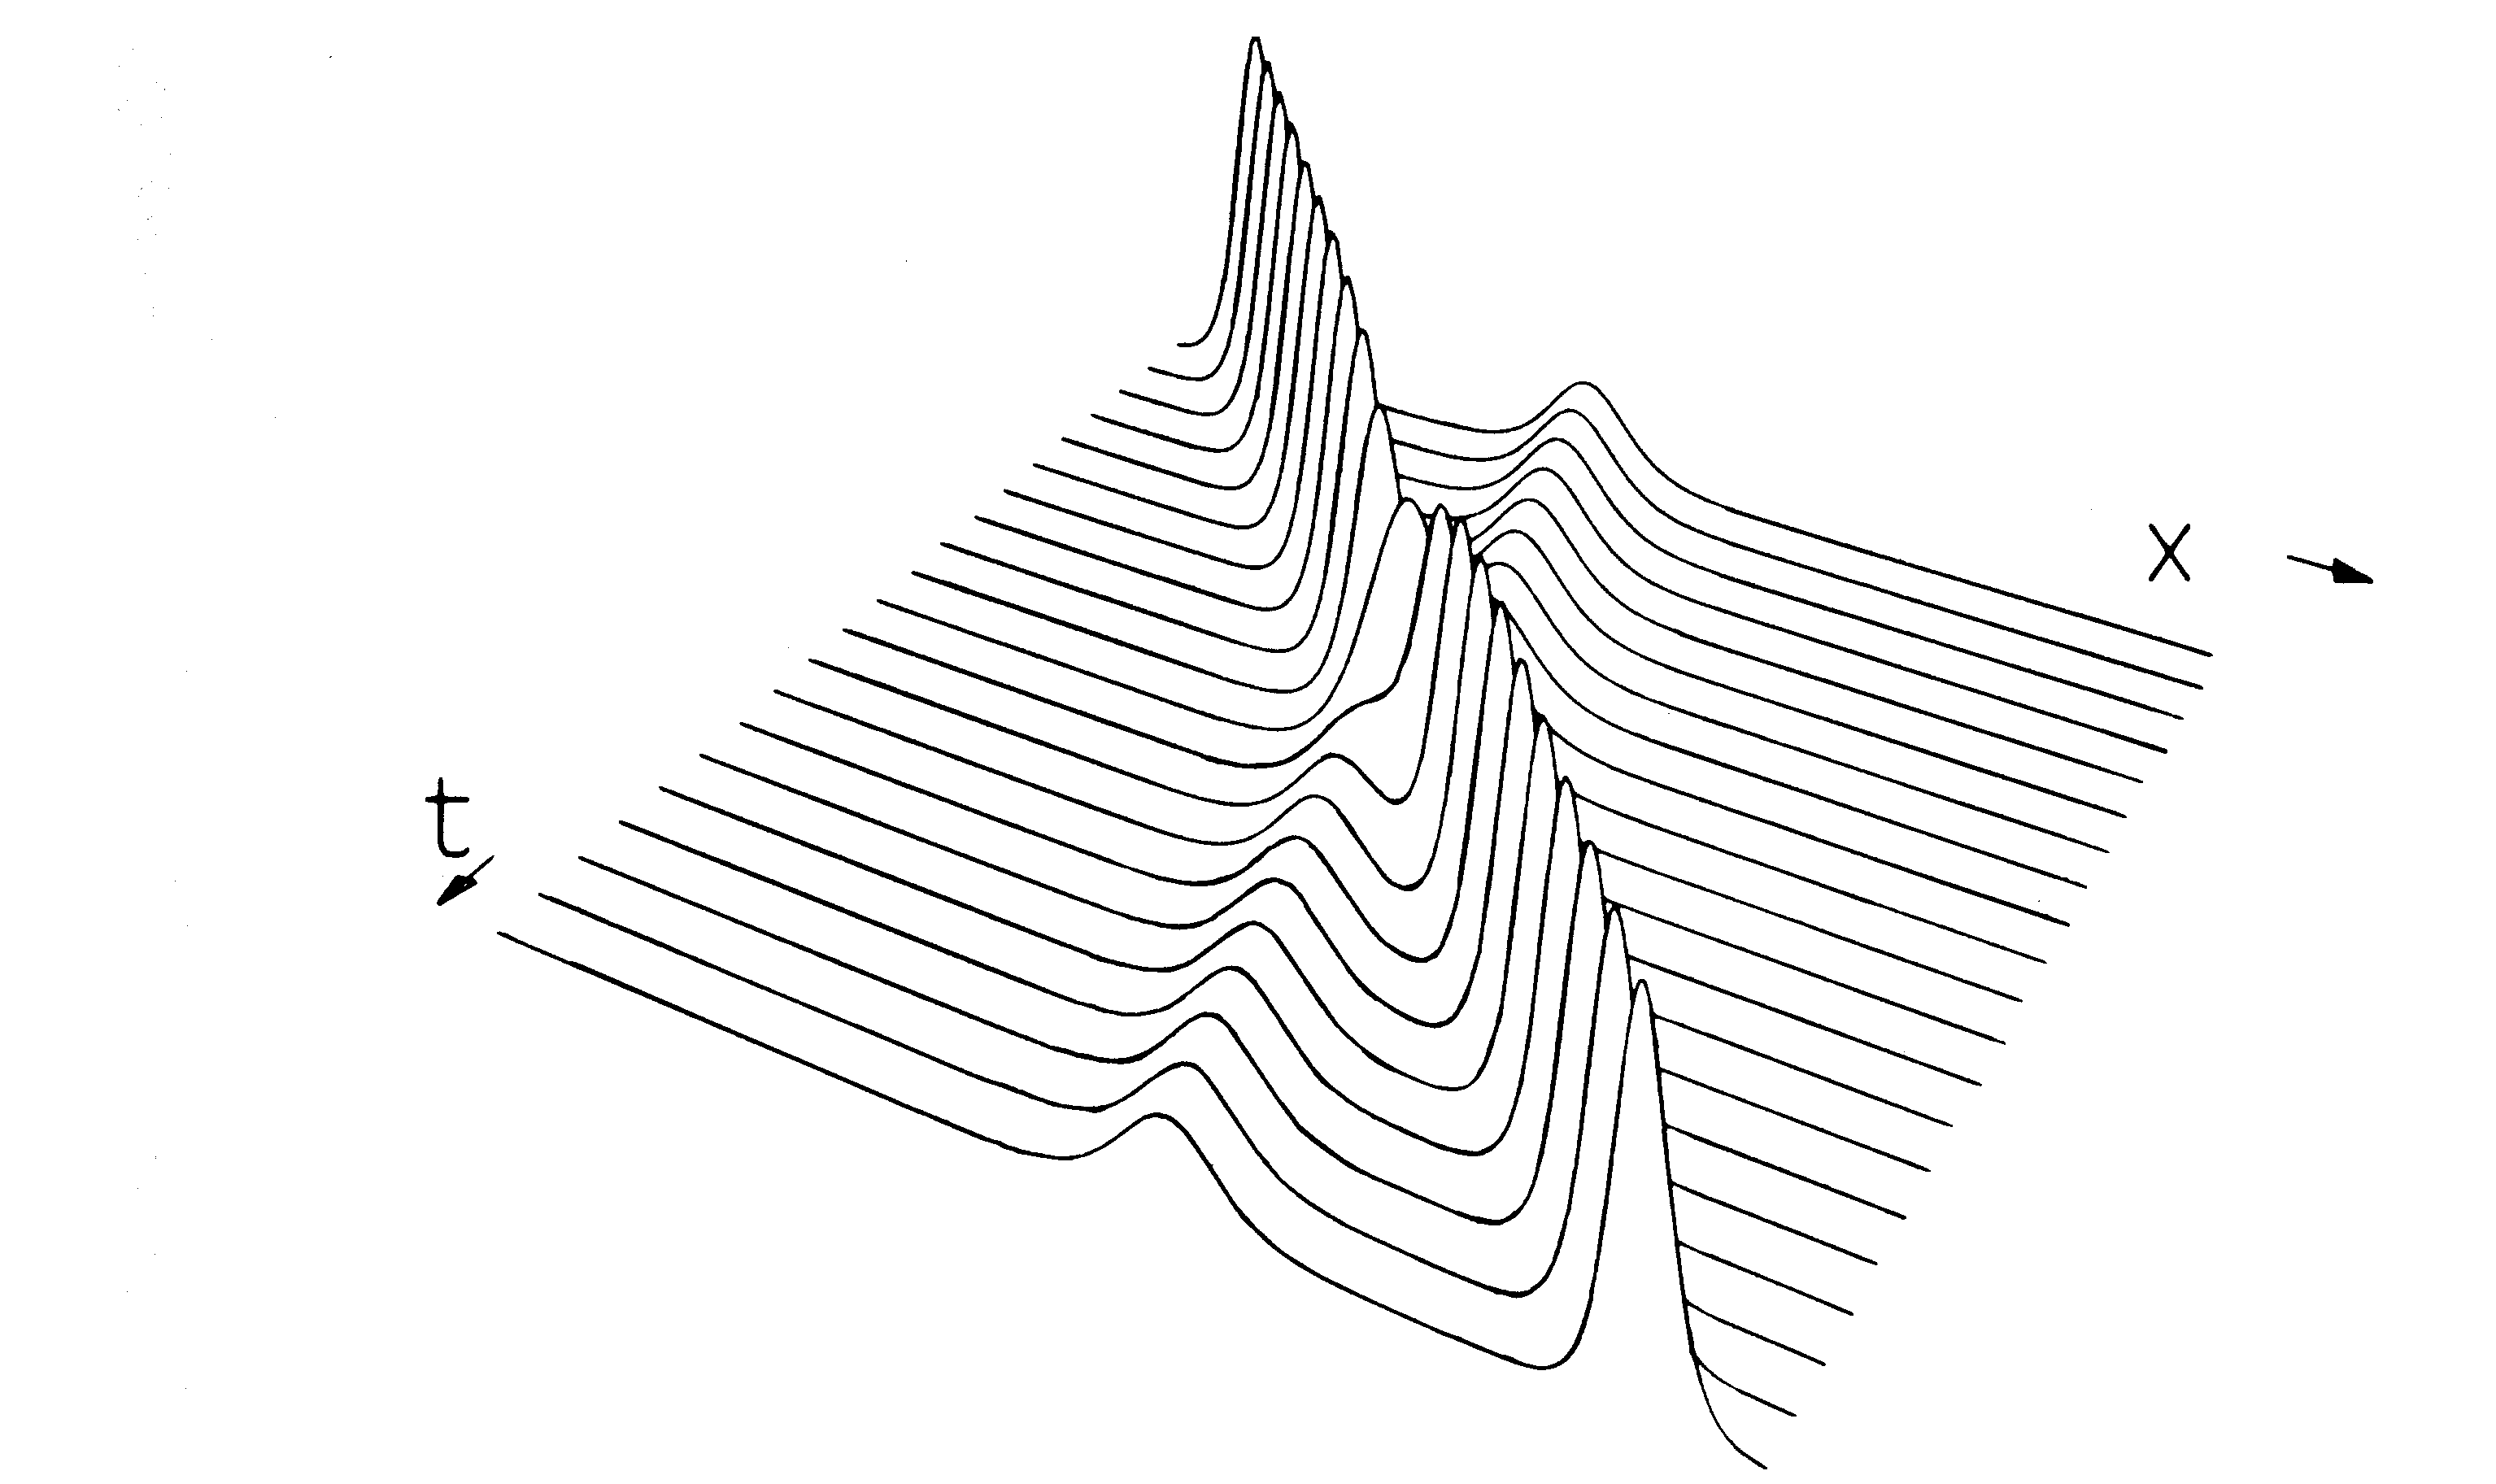
\includegraphics[width=0.6\linewidth]{kdv_collision.png}
	\caption{Попутное столкновение двух солитонов (из книги Р. Додда~\cite{Dodd}).}
	\label{fig:kdv_collision}
\end{figure}

Работа Забужского и Краскала дала толчок к аналитическим исследованиям уравнения Кортевега-де Фриза (КдФ), которые привели к возникновению в 1967 году метода обратной задачи рассеяния (МОЗР), позволяющего получить точное аналитическое решение уравнения по заданному начальному условию~\cite{GardnerIST}. Позже этот метод был обобщён и на некоторые другие нелинейные волновые уравнения, однако лишь очень небольшое количество нелинейных систем являются полностью интегрируемыми (решаемыми с помощью МОЗР)~\cite{Zakharov}.

Для численного эксперимента в работе 1965 года Забужский и Краскал использовали простейшую явную конечно-разностную схему второго порядка по временной и пространственной переменной. Впоследствии был предложен ряд других более сложных неявных конечно-разностных схем и псевдоспектральных методов, обзору которых посвящена работа~\cite{Taha}. Численное моделирование особенно важно для неинтегрируемых систем, к числу которых относятся, например, все уравнения типа Буссинеска, кроме \eqref{1_boussinesq}. Для таких уравнений были предложены конечно-разностные схемы, в которых на каждом шаге для обработки нелинейного слагаемого проводится несколько внутренних итераций~\cite{Christov, Kolkovska}.
Помимо метода конечных разностей к нелинейным уравнениям применяют и другие численные методы, например, конечных объёмов и конечных элементов~\cite{Dutykh_Boussinesq, Karczewska}. Отметим, что для численного решения уравнений, обладающих гладкими решениями, в областях простой геометрии одним из лучших методов является псевдоспектральный метод, широко применяющийся в нелинейных задачах~\cite{Gottlieb_Orszag, Canuto2007}.

%Семейство спектральных методов основано на поиске решения уравнений в некотором конечномерном пространстве функций. В качестве базиса могут быть выбран, например, базис Фурье (набор синусов и косинусов), набор многочленов Чебышёва первого рода или многочленов Лежандра. В настоящей работе исследуются динамические задачи, в которых неизвестная функция зависит как от временной, так и от пространственных переменных: $u = u(x, t)$. Спектральный базис вводится, как правило, только для пространственной дискретизации, тогда как для численного решения ОДУ по временной переменной используются стандартные методы, например, Рунге-Кутты 4-го порядка~\cite{Gottlieb_Orszag}. Существует три типа спектральных методов: метод Галёркина, тау метод и метод коллокаций (псевдоспектральный метод). Наиболее эффективным методом для решения нелинейных уравнений, а также уравнений с непостоянными коэффициентами является именно псевдоспектральный метод.


\section{Нелинейная динамика твёрдого тела}
В этом разделе приведены важные для дальнейшего изложения сведения по нелинейной динамике твёрдого тела, систематическому описанию которой посвящено множество книг, например,~\cite{LurieNL}. 

Динамика упругой сплошной среды, занимающей объём $\Omega$, описывается уравнениями движения, которые в векторном виде в случае однородного тела представляются следующим образом:
\begin{equation}\label{1_dynamics}
\rho\ddot{\vect{U}}(\vect{x}, t) = \divg \tens{P} + \vect{F}, \quad \vect{x}\in\Omega.
\end{equation}
Здесь $\rho$ -- плотность материала, $\vect{U}(\vect{x},t)$ -- вектор перемещений, $\vect{x}$ -- координаты точки среды в отсчётной конфигурации, $\tens{P}$ -- первый тензор напряжений Пиолы-Кирхгофа, $\vect{F}$ -- плотность массовых сил, точка обозначает взятие частной производной по времени, а дивергенция берётся по координатам в отсчётной конфигурации. Тензор напряжений $\tens{P}$ выражается через тензор деформации $\tens{E}$ следующим образом:
\begin{equation} \label{1_piola}
\tens{P} = (\tens{I} + \nabla\vect{U}) \cdot \pdiff{\Pi}{\tens{E}},
\end{equation}
где $\Pi$ -- плотность энергии деформации, а тензор деформации связан с градиентом перемещения:
\begin{equation}\label{1_strain}
2\tens{E} = (\nabla\vect{U})^T + \nabla\vect{U} + (\nabla\vect{U})^T\cdot\nabla\vect{U} \,.
\end{equation}
Заметим, что в линейной теории деформация предполагается бесконечно малой и нелинейное слагаемое в \eqref{1_strain} отбрасывается. Для завершения постановки задачи уравнения \eqref{1_dynamics} -- \eqref{1_strain} необходимо дополнить соотношением, связывающем энергию и деформацию, а также граничными условиями:
\begin{equation}\label{1_bc}
\vect{U} = \vect{U}_b, \;\; \vect{x}\in S_U; \qquad \tens{P}\cdot\vect{n} = \vect{P}_b, \;\; \vect{x}\in S_P; \qquad S_U\cup S_P = \partial\Omega.
\end{equation}
%Случай, когда $\vect{P}_b = 0$ будем называть условием свободной поверхности.

Энергия деформации $\Pi$ однородного и изотропного тела может быть разложена в ряд по инвариантам $I_i$ тензора деформации:
\begin{equation}\label{1_murnaghan}
\Pi = \frac{\lambda + 2\mu}{2}I_1(\tens{E})^2 - 2\mu I_2(\tens{E}) + \frac{l+2m}{3}I_1(\tens{E})^3 - 2m I_1(\tens{E}) I_2(\tens{E}) + n I_3(\tens{E}) + \dots,
\end{equation}
при этом коэффициенты в этом разложении характеризуют упругость материала и называются модулями упругости ($\lambda$ и $\mu$ -- коэффициенты Ламе, а $l$, $m$, $n$ -- модули Мурнагана). Заметим, что первые два слагаемых в приведённом разложении являются слагаемыми второго порядка относительно компонент тензора $\tens{E}$, а следующие три -- третьего порядка.
В разложении \eqref{1_murnaghan} для линейно упругого материала удерживаются только слагаемые второго порядка, а для слабо нелинейного материала Мурнагана~\cite{Murnaghan} учитываются ещё и слагаемые третьего порядка. Существуют другие нелинейно упругие материалы, например, материал Муни-Ривлина или Огдена, однако они предназначены в первую очередь для описания резиноподобных материалов, подверженных большим деформациям~\cite{Bergstrom}. Отметим, что нелинейно упругие материалы иногда называют гиперупругими.

Помимо классической постановки задачи в виде дифференциальных уравнений в частных производных \eqref{1_dynamics}, \eqref{1_bc}, существует вариационная постановка на основе принципа Гамильтона, гласящего, что истинная траектория системы $\vect{U}$ является стационарной точкой функционала действия $\mathcal{S}$:
\begin{equation}\label{1_action}
%\underset{\vect{U}\in W^1_2(\Omega, \mathbb{R}^3)}{\inf \mathcal{S},} \quad 
\delta\mathcal{S} = \delta\int_{t_1}^{t_2} dt \lsq \int_{\Omega} \lb \frac12\rho\dot{\vect{U}}^2 - \Pi + \vect{F}\cdot\vect{U} \rb dx + \int_{S_P} \vect{P}_b\cdot\vect{U} ds \rsq = 0.
\end{equation}
В \eqref{1_action} варьирование происходит по перемещениям $\vect{U}$. Отметим, что существует обобщённый принцип Гамильтона, где в функционал действия включаются соотношения \eqref{1_piola} и \eqref{1_strain}, а варьирование осуществляется не только по перемещениям, но и по деформациям $\tens{E}$ и напряжениям $\tens{P}$~\cite{Yu}.
%Отметим, что некоторые авторы использовали <<неполный>> принцип наименьшего действия, при котором в функционал действия включаются только уравнения движения (объёмный интеграл по $\Omega$), а граничные условия ставятся в виде уравнений \eqref{1_bc}.

%Упомянутые выше постановки задачи используют непрерывную модель твёрдого тела. Однако твёрдое тело можно описать дискретно с помощью решёточной модели~\cite{Maugin}, простейшая из которых -- цепочка грузов, соединённых пружинами -- представлена на рисунке \ref{fig:chain}.
%Определяя закон упругости пружины, то есть вводя потенциал взаимодействия между грузами, можно записать дискретные уравнения движения.


\section{Нелинейные волны деформации в твёрдых упругих волноводах}
%The study of nonlinear waves in solids is an important theme of the current research on waves (see, for example, \cite{Maugin,Dai,M,HL,E1,P,E2} and references therein). The research includes the studies of bulk strain solitons in solid waveguides (e.g. \cite{S_book,P_book}). Historically, theoretical developments began with the studies of waves in elastic rods of circular cross section. G.A. Nariboli and A. Sedov have systematically derived the Burgers - Korteweg de Vries equation for long longitudinal waves in a viscoelastic rod using power series expansions in the radius \cite{NS}. Later, L.A. Ostrovsky and A.M. Sutin have developed a regularised Boussinesq - type model using the plane cross section and Love's hypothesis in order to simplify the Lagrangian of the problem \cite{OS}. 

%Изучение нелинейных волн деформации в твёрдых телах является важной темой современного изучения волн \cite{Maugin,Dai,M,HL,E1,P,E2}. Исследование включает в себя изучение солитонов деформации в твердотельных волноводах \cite{S_book,P_book}. 
Изучение нелинейных волн деформации в твёрдых телах, в том числе солитонов деформации, является важной темой современного изучения волн~\cite{S_book, P_book}.
Разработка теории началась в 1970\babelhyphen{nobreak}х годах с исследования волн в упругом стержне круглого сечения, поскольку такая геометрия волновода является наиболее простой.

Исторически первым исследованием стала работа Г.~Нариболи и А.~Седова, которым удалось вывести уравнение Бюргерса-Кортевега-де~Фриза для длинных продольных волн в бесконечном вязкоупругом осесимметричном стержне со свободной от напряжений поверхностью~\cite{NS}. Для этого уравнения нелинейной теории упругости~\eqref{1_dynamics} и граничные условия~\eqref{1_bc}, записанные в цилиндрической системе координат $(x,r,\varphi)$, были упрощены с помощью:
\begin{itemize}[noitemsep,topsep=1pt]
	\item предположения о малости радиуса стержня $a \ll 1$,
	\item разложения перемещений в степенной ряд по радиусу стержня: 
	\begin{align}\label{1_nariboli}
	U(x,r,t) &= U_0(x,t) + a^2 U_2(x,r,t) + \mathcal{O}(a^4),\\
	V(x,r,t) &= -a \nu r \pdiff{U_0}{x} + a^3 V_3(x,r,t) + \mathcal{O}(a^5),
	\end{align}
	где $U$ -- продольное перемещение вдоль оси стержня, совпадающей с осью $x$, $V$ -- радиальное перемещение, а $\nu$ -- коэффициент Пуассона,
	\item предположения о малых деформациях $U, \, V \sim \varepsilon \ll 1$.
\end{itemize}
Позже Л.~Островский и А.~Сутин получили модель типа Буссинеска, %:
%\begin{equation}\label{1_ostrovsky_bou}
%u_{tt} - u_{xx} - 3 (u^2)_{xx} - u_{ttxx} = 0,
%\end{equation}
используя принцип Гамильтона и нижеследующие гипотезы, позволившие упростить функционал действия задачи~\cite{OS}: 
\begin{equation}\label{1_ostrovsky_hyp}
U(x,r,t) = U(x,t), \qquad V(x,r,t) = -\nu r \pdiff U x.
\end{equation}
Первая из этих гипотез называется гипотезой плоских сечений и означает, что поперечные сечения стержня остаются плоскими после деформации, а вторая гипотеза аналогична гипотезе Кирхгофа-Лява в теории тонких пластин и оболочек~\cite{Love}.
%A.M. Samsonov has suggested a model with two types of dispersive terms  \cite{S1}, and a model for the rod with a variable radius and elastic moduli \cite{S2}. The coefficients of Samsonov's model with two types of dispersive terms have been refined in the works by A.M. Samsonov and A.V. Porubov  \cite{SP, S_book, P_book}, and a dispersive-dissipative model has been suggested by A.V. Porubov and M.G. Velarde \cite{PV}. A model with three types of dispersive terms has been discussed by V.I. Erofeev et al. (see \cite{E_book} and references therein), however, the nonlinearity coefficient of this model differs from that in the  models of L.A. Ostrovsky and A.M. Sutin, and A.M. Samsonov and A.V. Porubov, while the choice of dispersive coefficients has not been fixed.
А.\,М.~Самсонов, используя подход Островского и Сутина, предложил модель типа Буссинеска с двумя дисперсионными слагаемыми и обобщил её на случай с меняющимися вдоль оси стержня радиусом и модулями упругости~\cite{S1, S2}. Коэффициенты модели Самсонова с двумя типами дисперсионных членов были позже уточнены в работах А.\,М.~Самсонова и А.\,В.~Порубова~\cite{SP}.
А.\,В.~Порубовым и М.~Веларде предложена дисперсионно-диссипативная модель для длинных волн в упругом стержне, помещённом в вязкоупругую среду~\cite{PV}.
Модель типа Буссинеска с тремя типами дисперсионных членов обсуждалась В.\,И.~Ерофеевым, однако коэффициент при нелинейном слагаемом в его модели отличается от соответствующего коэффициента у Островского и Самсонова~\cite{E_book}. Все выводы моделей типа Буссинеска в упомянутых исследованиях основывались на представлении Мурнагана для энергии упругой деформации и последующем упрощении полного функционала действия задачи с использованием некоторых гипотез. 

Несколько другой подход к задаче применён в работе X. Дая и X. Фана, которым удалось упростить полные уравнения движения с граничными условиями в виде свободной от напряжений поверхности стержня, сведя их к системе из двух связанных уравнений~\cite{DF}. Для этого была введена система масштабов для переменных и функций так, что масштаб перемещений $h$ и радиус стержня $a$предполагались малыми по сравнению с характерной длиной волны~$l$: $\varepsilon = h/l \ll 1$, $\delta = a^2/l^2 \ll 1$.
%\begin{itemize}[noitemsep,topsep=1pt]
%	\item масштаб перемещений $h$ мал по сравнению с характерной длиной волны $l$: $\varepsilon = h/l \ll 1$,
%	\item радиус стержня $a$ мал по сравнению с характерной длиной волны $l$: $\delta = a^2/l^2 \ll 1$.
%\end{itemize}
Полные уравнения были упрощены при помощи разложения перемещений в степенной ряд по радиальной координате и отбрасывания членов порядка $\mathcal{O}(\varepsilon^2, \varepsilon\delta, \delta^2)$.
%Кроме того, были использованы разложения перемещений в ряд по радиальной координате. Упрощённые уравнения были выведены из полных с помощью метода регулярных возмущений и отбрасывания членов порядка $\mathcal{O}(\varepsilon^2, \varepsilon\delta, \delta^2)$.
В другой работе X.~Дай и З.~Цай применили аналогичный асимптотический вывод для описания волн в предварительно растянутом гиперупругом стержне, сделанном из материала Муни-Ривлина~\cite{DC}.

Во всех приведённых выше работах твёрдое тело считалось непрерывным. Однако помимо непрерывной модели существует решёточная (дискретная) модель, согласно которой твёрдое тело представляется в виде системы часиц некоторой массы, соединённых пружинами. В рамках такой модели К.\,Р. Хуснутдинова и др., предполагая пружины нелинейно упругими, получили систему разностно-дифференциальных уравнений, которая в континуальном пределе сводится к уравнению типа Буссинеска~\cite{KSZ}. Заметим, что уравнение модели было получено из полных уравнений движения с помощью асимптотических методов без использования упрощающих гипотез. Интересно, что в этом исследовании была выведена модель типа Буссинеска с тремя дисперсионными слагаемыми, а также система связанных уравнений типа Буссинеска для волн в слоистом волноводе с неидеальным контактом.
%К.Р. Хуснутдинова и соавторы рассмотрели ангармоническую цепочку осциллирующих диполей и вывели систему разностно-дифференциальных уравнений движения~\cite{KSZ}. Эта система в континуальном пределе, используя масштабирование, выделяющее продольные волны, была сведена к уравнению типа Буссинеска.
В недавних исследованиях модели типа Буссинеска использовались для изучения распространения длинных продольных уединённых волн деформации в волноводе с расслоением \cite{KS, KT1, KT2}, а некоторые соответствующие экспериментальные наблюдения были опубликованы в \cite{JAP2010, JAP2012}. 
%Отметим исследования по распространению нелинейных волн на дефектах в решетках \cite{ML} и струнах \cite{AM}. Некоторые другие модели типа Буссинеска были получены для описания распространения поперечных волн большой амплитуды~\cite{DS}.

Целью настоящей работы является исследование длинных продольных слабонелинейных волн деформации в круглом бесконечном стержне методами асимптотического анализа и численного моделирования. Исследователи, занимавшиеся этой задачей ранее, полагали боковую поверхность стержня свободной от напряжений, поэтому научный интерес представляет обобщение вывода модели типа Буссинеска на случай, когда имеется ненулевая осесимметричная нагрузка на боковой поверхности, а также продольное предварительное растяжение стержня.
%Научный интерес представляет задача с ненулевой осесимметричной нагрузкой на боковой поверхности стержня, поскольку исследователи, занимавшиеся этой задачей ранее, полагали её свободной от напряжений. 
Большое значение имеет построение численной схемы решения полных нелинейных уравнений динамики упругого стержня, поскольку она может служить средством для верификации упрощённых моделей и более детального исследования нелинейных волн.

Вывод моделей в настоящей работе выполнен с помощью пакета символьных вычислений Mathematica, а результаты работы частично опубликованы автором в сотрудничестве с К.\,Р.~Хуснутдиновой и И.\,В.~Семёновой~\cite{Garbuzov}.
%Для этого с помощью методов асимптотического анализа производится упрощение полных уравнений динамики упругого тела и сведение их к одному уравнению типа Буссинеска, где, в отличие от других работ, учтена ненулевая осесимметричная нагрузка на боковой поверхности и продольное предварительное растяжение.
%Для этого используются как методы асимптотического анализа, позволяющие из полных уравнений деформации стержня получить упрощённую модель типа Буссинеска и Кортевега-де Фриза, так и численные методы. 

%Цель настоящей работы -- вернуться к выводу слабо нелинейной длинноволновой модели для продольных волн в круглом бесконечном стержне, чтобы 
%систематически 
%получить новую модель типа Буссинеска и распространить её на более сложный случай, когда имеется ненулевая осесимметричная нагрузка на боковой поверхности и продольное предварительное растяжение. 
%Вывод модели осуществляется с помощью пакета MATHEMATICA.
%Кроме этого, в настоящей работе обсуждаются основные решения в виде уединённых волн, а также дисперсионные свойства описанных здесь моделей. Результаты этой работы опубликованы автором в сотрудничестве с К.Р. Хуснутдиновой и И.В. Семёновой~\cite{Garbuzov}.

%All derivations of Boussinesq-type models in these studies were based on the use of the Murnaghan model for elastic energy \cite{Murnaghan}, accounting for both physical and geometrical sources of nonlinearity, and subsequent simplification of the full Lagrangian of the problem using some hypothesis. In \cite{DF} {\color{red} H.-H. Dai and X. Fan have obtained} a system of two coupled equations and a uni-directional model of the Benjamin-Bona-Mahony (BBM) type within the scope of nonlinear elasticity, using a systematic asymptotic derivation from the full equations of motion and free surface boundary conditions. The systematic asymptotic analysis has been also developed for the description of linear transient waves in a pre-stretched compressible hyperelastic material (with application to Mooney-Rivlin material) in \cite{DC}. In  \cite{KSZ}, a Boussinesq-type model 
%for a nonlinearly elastic waveguide with both physical and geometrical sources of nonlinearity 
%has been derived using  the systematic asymptotic derivation within the scope of a lattice model, i.e. the model equation has been derived from the full equations of motion, and no hypothesis have been used to simplify the Lagrangian of the problem. Interestingly, Boussinesq-type models with both two and three types of dispersive terms have been systematically derived in the latter study, as well as coupled Boussinesq-type equations for the waves in a layered waveguide with an imperfect interface.
%
%The Boussinesq-type models have been recently used to study the scattering of long longitudinal bulk strain solitary waves by delamination in \cite{KS,KT1, KT2}, and some related experimental observations have been reported in \cite{JAP2010, JAP2012}. We also note the related studies on nonlinear wave scattering by defects in lattices \cite{ML} and strings \cite{AM}. {\color{red} Some other Boussinesq-type models have been derived to describe the propagation of large amplitude transverse waves (see \cite{DS} and references therein).}
%
%The aim of our current paper is to revisit the derivation of nonlinear two-directional long wave models  for longitudinal waves within the scope of nonlinear dynamic elasticity in order to systematically derive a Boussineq-type model, 
%%i.e. from the full equations of motion and boundary conditions using asymptotic expansions in the powers of two small parameters present in the problem, 
%and  to extend these derivations to the more complicated case when there is non-zero axisymmetric loading on the boundary surface, and a background longitudinal pre-stretch.
%%We do not impose any ad hoc hypothesis to simplify the Lagrangian. 
%The derivations are performed using symbolic computations with MATHEMATICA \cite{Mathematica}. We also discuss the basic solitary wave solutions  and dispersive properties of the models.
%%and develop an efficient pseudospectral approach to numerical simulations with the derived equations. 
%Finally, we briefly describe the experiments on generation of solitary waves in the Ioffe Institute by the group which was headed by Alexander M. Samsonov, and suggest that our derived models will be useful for the mathematical modelling of the generation processes. This paper is dedicated to the memory of our dear colleague and friend.



\chapter{Слабо нелинейные продольные волны деформации в тонких волноводах}

\section{Формулировка задачи}

%We consider a rod of circular cross section with the radius $R$ and use cylindrical coordinates $(x, r, \varphi)$ with the axial coordinate $x$, radial coordinate $r$ and angular coordinate $\varphi$. We use the Lagrangian description and denote the displacement vector by $\underline{U} = (U, V, W) $, where $ U $ is the axial displacement, $ V $ is the radial displacement and $ W $ is the torsion. 

Рассмотрим стержень круглого поперечного сечения радиуса $R$. Введём цилиндрическую систему координат $(x, r, \varphi)$, где $x$ -- осевая координата, $r$ -- продольная, $\varphi$ -- угловая, как показано на рисунке \ref{fig:rod}. Положим стержень бесконечным вдоль оси $x$. Используя Лагранжев подход, введём вектор перемещения точек тела: $\vect{U} = (U, V, W)$, где $U$ -- осевое (продольное) перемещение, $V$ -- радиальное (поперечное) перемещение, а $W$ -- вращение.
\begin{figure}[h]
	\centering
	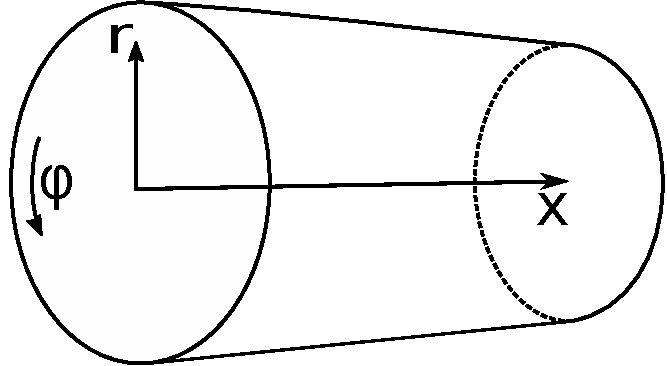
\includegraphics[width=0.33\textwidth]{Fig1}
	\caption{Стержень с круглым поперечным сечением.}
	\label{fig:rod}
\end{figure}

Следуя предыдущим исследованиям, которые обсуждались в главе 1, будем рассматривать стержень, сделанный из материала Мурнагана, энергия упругой деформации которого представляется в виде:
%Similarly to the previous studies discussed in the Introduction we assume that the rod is made of a Murnaghan's hyperelastic material (\cite{Murnaghan}, see also \cite{S_book} and references therein). The strain energy density of that material can be written as
\begin{equation}\label{2_murnaghan_pot}
\Pi = \frac{\lambda + 2\mu}{2}I_1(\tens{E})^2 - 2\mu I_2(\tens{E}) + \frac{l+2m}{3}I_1(\tens{E})^3 - 2m I_1(\tens{E}) I_2(\tens{E}) + n I_3(\tens{E}),
\end{equation}
где $I_1(\tens{E}) = \trace \tens{E},\  I_2(\tens{E}) = \lsq(\trace \tens{E})^2 - \trace \tens{E}^2\rsq/\,2,\ I_3(\tens{E}) = \trace \tens{E}$ являются инвариантами тензора деформации Грина
$\tens{E} = \lb (\nabla\vect{U})^T + \nabla\vect{U} + (\nabla\vect{U})^T\cdot\nabla\vect{U} \rb / \, 2$, 
$\lambda$,~$\mu$ -- коэффициенты Ламе, $l$,~$m$,~$n$ -- модули Мурнагана. Здесь и далее в тексте работы все частные производные берутся по координатам в отсчётной конфигурации. Отметим, что модель Мурнагана является общей моделью слабо нелинейных упругих деформаций.
%Here, and in the following, all spatial derivatives are taken with respect to the natural (underformed) coordinates {\color{red} in the reference configuration. It is worth noting that the Murnaghan model is used here in the sense of the general weakly-nonlinear theory of elasticity, assuming small values of strain (see the discussion in \cite{DSS}).}


%The equations of motion are given by
%\begin{equation}
%\rho\  \ddot {\vect{U}} = {\rm div}\ \tens{P},
%\label{P}
%\end{equation}
%where $\rho$ is the material density in the natural configuration, dots denote differentiation with respect to time, and $ \tens{P} $ is the first Piola-Kirchhoff stress tensor 
%\begin{equation}\label{piola-k}
%\tens{P} =  (I + \nabla\vect{U}) \cdot \frac{\partial\Pi}{\partial\tens{E}}.
%\end{equation} 

Рассмотрим задачу, в которой отсутствует кручение стержня, а продольное и поперечное перемещения $U$ и $V$ не зависят от угла $\varphi$:
%We now consider an exact reduction of the full equations of motion describing solutions with no torsion ($W=0$), and where the longitudinal and transverse displacements $U$ and $V$ are independent of $ \varphi $:
\begin{equation}\label{2_assumptions}
U = U(x,r,t), \quad V = V(x,r,t), \quad W = 0.
\end{equation}
Уравнения движения, в условиях \eqref{2_assumptions} и отсутствия массовых сил, принимают вид
\begin{align}
\label{2_eq1_0}
&\rho  \frac{\partial^2 U(x,r,t)}{\partial t^2}-\frac{\partial P_{x x}}{\partial x}-\frac{\partial P_{xr}}{\partial r}-\frac{P_{xr}}{r} = 0,\\
\label{2_eq2_0}
&\rho  \frac{\partial^2 V(x,r,t)}{\partial t^2} - \frac{\partial P_{rx}}{\partial x}-\frac{\partial P_{rr}}{\partial r}-\frac{P_{rr} - P_{\varphi\varphi}}{r} = 0,
\end{align}
а третье уравнение представляется в виде тождества $0\equiv 0$. Здесь $P_{\alpha \beta}$ обозначает компоненту первого тензора Пиолы-Кирхгофа, а $\rho$ -- плотность материала.
%while the third equation is identically satisfied. Here, $P_{\alpha \beta}$ denote components of the first Piola-Kirchhoff stress tensor, {\color{red} and we do not use different fonts for the coordinates in the current and reference configurations in these notations.}

Зададим на поверхности стержня осесимметричное напряжение $\vect{P_b} = (P(x,t), T(x,t), 0)$. Тогда граничные условия имеют вид:
%The equations of motion are complemented by the surface boundary conditions
%\begin{equation} \label{2_bc}
%\tens{P}\cdot \vect{n} = \vect{P_b} = (P(x,t), T(x,t), 0),
%\end{equation}
%где $\vect{n}$ -- нормаль к поверхности. Следовательно, граничные условия представляются в виде
%where $\vect{n}$ is the normal vector to the lateral surface, and $\vect{P_b} = (P(x,t), T(x,t), 0)$, i.e. we consider the rotationally symmetric case, and $P(x,t)$ and $T(x,t)$ are the known tractions.
%Thus, the boundary conditions are given by
\begin{align}
P_{rr} &= P(x, t) \quad \mbox{при} \quad r = R \label{2_bc_rr},\\
P_{xr} &= T(x, t) \quad \mbox{при} \quad r = R \label{2_bc_rx}.
\end{align}
Поскольку компонента $ P_{\varphi r} \equiv 0 $, третье граничное условие $P_{\varphi r} = 0$ при $r = R$ выполняется автоматически.


\section{Вывод уравнения типа Буссинеска с внешним воздействием} 
\subsection{Вывод с помощью степенных разложений по радиусу}
\label{sec:derivation}
%\label{s:power_series_exp}
Подход к выводу уравнения модели в этом разделе опирается на метод, описанный в~\cite{DF}. Упростим этот метод с помощью разложений, использованных для вывода линейной модели~\cite{bostrm2000}. Таким образом, будем искать решение в виде степенного ряда по радиальной координате:
%Our approach  to the derivation of the model equation in this section is essentially similar to the derivation in \cite{DF}, but we simplify it by adopting expansions used in the derivation of the linear model in \cite{bostrm2000}. Thus, we look for a solution of the  problem in the form of power series expansions of the displacements in the radial coordinate:
\begin{align}
\label{u_series}
U(x,r,t) &= U_0(x,t) + r^2 U_2(x,t) + r^4 U_4(x,t) + \dots \, ,\\
\label{v_series}
V(x,r,t) &= r V_1(x,t) + r^3 V_3(x,t) + r^5 V_5(x,t) + \dots \, .
\end{align}
Отметим, что продольное перемещение разложено в ряд по чётным степеням радиуса, в то время как поперечное перемещение по нечётным. В линейной задаче такие разложения приняты потому, что, если учесть все степени в разложении, то уравнения движения \eqref{2_eq1_0}, \eqref{2_eq2_0} разобьются на две независимые системы уравнений. В первую систему войдут слагаемые $U_{2k}$ и $V_{2k+1}$, а во вторую $U_{2k+1}$ и $V_{2k}$ ($k \geqslant 0$). Для продольных волн в осесимметричном стержне должны выполняться очевидные условия:
\begin{equation}\label{2_longitud_cond}
\pdiff{U}{r} = 0, \quad V = 0 \quad \text{при} \quad r = 0,
\end{equation}
из которых следует, что $U_1 = V_0 = 0$. В линейной задаче из равенства нулю этих двух слагаемых автоматически следует, что все слагаемые $U_{2k+1}$ и $V_{2k}$ тоже равны нулю. Для нелинейной задачи тоже можно показать справедливость этого утверждения, однако, чтобы не слишком усложнять вывод, примем эти разложения в качестве допущения. Кроме того, в отличие от~\cite{DF}, мы сведём задачу к одному уравнению типа Буссинеска, учтём ненулевое осесимметричное напряжение, приложенное к поверхности стержня, а также рассмотрим предварительно растянутый стержень.

Введём масштабные множители, выделяющие среди прочих задачу о распространении длинных по сравнению с радиусом стержня волн малой амплитуды. Тогда безразмерные переменные и функции определяются следующими выражениями:
%Рассмотрим длинные по сравнению с радиусом стержня волны малой амплитуды. Для этого введём масштабные множители и безразмерные переменные и функции:
\begin{equation} \label{scales1}
\tilde t = \frac{t}{L/c}, \quad \tilde x = \frac{x}{L}, \quad \tilde r = \frac{r}{L}, \quad \tilde U = \frac{U}{\varepsilon L}, \quad \tilde V = \frac{V}{\varepsilon L}, \quad \tilde P = \frac{P}{E \varepsilon}, \quad \tilde T = \frac{T}{E \varepsilon\delta},
\end{equation}
из которых следует, что
%which yields
$\displaystyle \tilde U_n =  \frac{L^n U_n}{\varepsilon L},  \ \tilde V_n =  \frac{L^n V_n}{\varepsilon L}$ для $n \geqslant 0$.
Здесь $L$ является характерной длиной волны, $c$ -- скорость линейной волны, $E$ -- модуль Юнга, $\varepsilon \ll 1$ -- малый параметр амплитуды, $\displaystyle \delta = \frac{R}{L} \ll 1$ -- второй малый параметр, а тильда обозначает безразмерную величину. Вспомним, что модуль Юнга и коэффициент Пуассона выражаются через коэффициенты Ламе:
%assuming that $L$ is the characteristic wavelength, $c$ is the linear wave speed, $E$ is the Young modulus, $\varepsilon$ is the small amplitude parameter (characterising the longitudinal strain), and $\displaystyle \delta = \frac{R}{L} $ is the second small parameter (long wavelength parameter). Here, the tilde denotes dimensionless variables and tractions. {\color{red} We are also interested in the equation for the case of weak tractions, which can be obtained by rescaling $\tilde P$ and $\tilde T$ in the derived equation.}  In the following we will use the expressions for the Young modulus and the Poisson ratio in terms of the Lame coefficients:
\begin{equation}\label{young_mod}
E = \frac{\mu(3\lambda + 2\mu)}{\lambda + \mu}, \quad \nu = \frac{\lambda}{2 (\lambda + \mu)}.
\end{equation}
С учётом \eqref{scales1} разложения \eqref{u_series}, \eqref{v_series} представляются в виде:
%Then, the expansions \eqref{u_series} and \eqref{v_series} take the form
\begin{align}
\label{u_series_scaled}
\widetilde U(\tilde x, \tilde r, \tilde t) &= \widetilde{U}_0(\tilde x, \tilde t) + \tilde{r}^2\widetilde{U}_2(\tilde x, \tilde t) + \tilde{r}^4\widetilde{U}_4(\tilde x, \tilde t) + O(\tilde r^6),\\
\label{v_series_scaled}
\widetilde V(\tilde x, \tilde r, \tilde t) &= \tilde{r} \widetilde{V}_1(\tilde x, \tilde t) + \tilde{r}^3\widetilde{V}_3(\tilde x, \tilde t) + \tilde{r}^5\widetilde{V_5}(\tilde x, \tilde t) + O(\tilde r^7).
\end{align}
%We consider only long waves in a thin rod, hence parameter $\delta$ is small: $ \delta \ll 1 $. By choice of the scales \eqref{scales} we assume that the %displacement components are slowly varying functions of the radial coordinate.
%In what follows we omit the tildes.
Радиальная координата $\tilde r$ точек стержня принимает значения от $0$ до $\delta$ и, следовательно, является малой величиной.
%Мы рассматриваем длинные волны в тонком стержне, следовательно, радиальная переменная меняется от 0 до $\delta$
В дальнейшем мы опустим тильду над безразмерными величинами.

Подставляя \eqref{u_series_scaled} и \eqref{v_series_scaled} в уравнения движения \eqref{2_eq1_0}, \eqref{2_eq2_0}, получаем
\begin{equation} 
\label{eq1_1}
\begin{split}
	&\rho c^2 U_{0tt} - (\lambda + 2\mu) U_{0xx} - 2(\lambda + \mu) V_{1x} - 4\mu U_2 + \Phi_1(U_0, V_1, U_2) \varepsilon\\
	&\qquad+ \left[\rho c^2 U_{2tt} - (\lambda + 2\mu)U_{2xx} - 4(\lambda + \mu)V_{3x} - 16\mu U_4\right] r^2 + O(\varepsilon^2, \varepsilon r^2, r^4) = 0,
\end{split}
\end{equation}
\begin{equation} \label{eq2_1}
\begin{split}
	&r \big( \rho c^2 V_{1tt} - \mu V_{1xx} - 2(\lambda + \mu)U_{2x} - 8(\lambda + 2\mu)V_3 - \Phi_2(U_0, V_1, U_2, V_3)\varepsilon \\
	&\qquad- \left[\rho c^2 V_{3tt} - \mu V_{3xx} - 4(\lambda + \mu)U_{4x} - 24(\lambda + 2\mu)V_5 \right] r^2  + O(\varepsilon^2, \varepsilon r^2, r^4)\big) = 0,
\end{split}
\end{equation}
где индексы $x$ и $t$ обозначают частные производные по соответствующим переменным, а выражения для нелинейных функций $\Phi_1$ и $\Phi_2$ приведены в Приложении~1.
Функции $ U_2 $, $ V_3 $, $ U_4 $ могут быть получены из \eqref{eq1_1} и \eqref{eq2_1}, приравнивая к нулю коэффициенты при различных степенях~$r$:
%The functions $ U_2 $, $ V_3 $, $ U_4 $ can be obtained from \eqref{eq1_1} and \eqref{eq2_1} by equating to zero the coefficients at different powers of $\delta$, and they have the following form:
\begin{align}
\label{U2}
U_2 &= \frac{1}{4\mu} \left[ \rho c^2 U_{0tt} - (\lambda + 2\mu) U_{0xx} - 2(\lambda + \mu) V_{1x} \right] + \varepsilon f_2(x,t) + O(\varepsilon^2),\\
\label{V3}
V_3 &= \frac{1}{8(\lambda + 2\mu)} \left[ \rho c^2 V_{1tt} - 2(\lambda + \mu) U_{2x} - \mu V_{1xx} \right] + \varepsilon f_3(x,t) + O(\varepsilon^2),\\
\label{U4}
U_4 &= \frac{1}{16\mu}\left[\rho c^2 U_{2tt} - (\lambda + 2\mu) U_{2xx} - 4(\lambda + \mu) V_{3x}\right] + O(\varepsilon).
%V_5 &=& \frac{1}{24(\lambda + 2\mu)} \left(\rho c^2 V_{3tt} - 4(\lambda+\mu)U_{4x} - \mu V_{3xx}\right) + O(\varepsilon).
\end{align}
Выражения для функций $f_2$ и $f_3$ приведены в Приложении 1.

Затем, подставляя функции $ U_2 $, $ V_3 $, $ U_4 $ в граничные условия \eqref{2_bc_rr}, \eqref{2_bc_rx}, которые в безразмерном виде должны выполняться при $r = \delta$, получаем уравнения:
\begin{equation} \label{2_bc_rr_subst}
\begin{split}
2 (\lambda + \mu) V_1 + \lambda U_{0x} &+\varepsilon \Psi_1(U_0, V_1) + \frac{\delta^2}{8} \bigg[ (\lambda + 3\mu) U_{0xxx}- \frac{\rho c^2(\lambda + 3\mu)}{\lambda + 2\mu} U_{0xtt} \\
&+ \frac{2\rho c^2(2\lambda + 3\mu)}{\lambda + 2\mu} V_{1tt} + 2\lambda V_{1xx}\bigg] 
+ O(\varepsilon^2, \varepsilon\delta^2, \delta^4) =  \frac{\mu(3\lambda + 2\mu)}{\lambda + \mu} P,
\end{split}
\end{equation}
\begin{equation} \label{2_bc_rx_subst}
\begin{split}
\rho  c^2 U_{0tt} -2 \lambda  V_{1x}-(\lambda +2 \mu ) U_{0xx} - \varepsilon \Psi_2(U_0, V_1)
+ \frac{\delta^2}{8}\bigg[(3\lambda + 4\mu)U_{0xxxx} + \frac{\rho^2 c^4}{\mu}U_{0tttt}\\
- \frac{\rho c^2\left(\lambda^2 + 7\lambda\mu + 8\mu^2\right)}{\mu(\lambda + 2\mu)} U_{0xxtt} + 2(3\lambda + 2\mu)V_{1xxx} - \frac{2 \rho  c^2 \left(\lambda ^2+4 \lambda  \mu +2 \mu ^2\right)}{\mu(\lambda + 2\mu)} V_{1xtt} \bigg]\\
+\,O(\varepsilon^2, \varepsilon\delta^2, \delta^4)
= \frac{2\mu(3\lambda + 2\mu)}{\lambda + \mu} T,
\end{split}
\end{equation}
где нелинейные члены выражаются следующим образом: 
\begin{align}
	\nonumber
	\Psi_1 &= (4l + 2m + 3\lambda + 3\mu) V_1^2 + (4l - 2m + n + \lambda) U_{0x} V_1 + \frac{1}{2} (2l + \lambda) U_{0x}^2, \\
	\nonumber
	\Psi_2 &= \left((4l - 2m + n + \lambda) V_1^2 + 2(2l + \lambda) U_{0x} V_1 + \frac12(2l + 4m + 3\lambda + 6\mu) U_{0x}^2 \right)_x.
\end{align}
Отметим, что при $\varepsilon = 0$ уравнения \eqref{2_bc_rr_subst} и \eqref{2_bc_rx_subst} сводятся к уравнениям, полученным в линейной задаче~\cite{bostrm2000}. Эта система связанных уравнений представляет собой довольно сложную модель, однако она может быть сведена к одному уравнению типа Буссинеска.

Существует два естественных способа вывода модели типа Буссинеска. В первом способе исключение функции $V_1$ из уравнений \eqref{2_bc_rr_subst} и \eqref{2_bc_rx_subst} осуществляется с помощью асимптотического выражения, следующего из уравнения \eqref{2_bc_rr_subst}:
\begin{equation} \label{v1_asympt}
V_1(x, t) = \frac{ \mu(3\lambda + 2\mu) P - \lambda(\lambda + \mu) U_{0x}}{2(\lambda + \mu)^2} + \varepsilon f(x,t) + \delta^2 g(x,t) + O(\varepsilon^2, \varepsilon\delta^2, \delta^4),
\end{equation}
где неизвестные функции $f$ и $g$ ищутся из условия равенства нулю коэффициентов при $\varepsilon$ и $\delta^2$ в \eqref{2_bc_rr_subst}. Их вид представлен в Приложении 1. Затем, подстановка $V_1$ в \eqref{2_bc_rx_subst} приводит к следующему уравнению типа Буссинеска относительно $U_0$:
\begin{equation} \label{eq_u0_asympt}
\begin{split}
\rho c^2 U_{0tt} &- \frac{\mu(3\lambda + 2\mu)}{\lambda + \mu}\left(U_{0xx} + \frac{\lambda}{\lambda + \mu} P_x + 2T\right) - \varepsilon \left(\gamma_1 U_{0x}^2 + \gamma_2 U_x P + \gamma_3 P^2 \right)_x \\
&+ \delta^2 \bigg[\frac{\rho ^2 c^4 U_{0tttt}}{8\mu} + \frac{\mu (3\lambda + 2\mu)^2 U_{0xxxx}}{8(\lambda + \mu)^2} - \frac{\rho c^2 \left(7\lambda^2 + 10\lambda\mu + 4\mu^2\right) U_{0xxtt}}{8(\lambda + \mu)^2} + F \bigg]\\
&\hspace{100mm}+ O(\varepsilon^2, \varepsilon\delta^2, \delta^4) = 0.
\end{split}
\end{equation}
Здесь нелинейные коэффициенты $\gamma_i$ и функция $F$ представляются в виде:
\begin{align} 
	\nonumber
	\gamma_1 &= \frac{3n(\lambda + \mu)\lambda^2 + 2\mu \left[9\lambda^3 + 24\mu\lambda^2 + 21\mu^2\lambda + m(3\lambda + 2\mu)^2 + 2\mu^2 (l + 3\mu)\right]}{4 (\lambda + \mu)^3},\\
	\nonumber
	\gamma_2 &= \frac{\left[3\lambda^3 + 5\lambda^2\mu + 2\lambda\mu^2 + 4l\mu^2 + 2\lambda m(3\lambda + 2\mu) - 2\lambda n (\lambda + \mu)\right] \mu(3\lambda + 2\mu)}{2(\lambda + \mu)^4},\\
	\nonumber
	\gamma_3 &= \frac{\left[n (\lambda +\mu )-2 \left(\lambda ^2+\lambda  \mu -2 l \mu \right)-2 m (2 \lambda +\mu )\right] \mu^2 (3\lambda + 2\mu)^2}{4(\lambda + \mu)^5},\\
	\nonumber
	F &= \frac{3\lambda + 2\mu}{8\mu(\lambda + \mu)^3}\left[ \mu (4\lambda^2 + 5\lambda\mu + 2\mu^2) P_{xxx} - \rho c^2(\lambda^2 + \lambda\mu + \mu^2) P_{xtt}\right].
\end{align}

Другой метод основан на исключении $V_1$ из \eqref{2_bc_rr_subst} и \eqref{2_bc_rx_subst} таким образом, каким это сделано в~\cite{bostrm2000} для линейной задачи. В линейном случае этот подход не использует асимптотическое выражение \eqref{v1_asympt} и приводит к уравнению того же типа, что и \eqref{eq_u0_asympt}, но с другими коэффициентами при дисперсионных слагаемых. Действительно, уравнения \eqref{2_bc_rr_subst} и \eqref{2_bc_rx_subst} могут быть записаны в виде:
\begin{align}%\label{key}
L_{1} V_1 + \varepsilon N_1(U_0, V_1, \dots) &= M_1(U_0, P, \dots) + O(\varepsilon^2, \varepsilon\delta^2, \delta^4),\\
L_{2} V_1 + \varepsilon N_2(U_0, V_1, \dots) &= M_2(U_0, T, \dots) + O(\varepsilon^2, \varepsilon\delta^2, \delta^4),
\end{align}
где $L_{1}$ и $L_{2}$ -- линейные дифференциальные операторы, действующие на $V_1$, а $N_1(U_0, V_1, \dots)$, $M_1 (U_0, P, \dots)$ и $N_2(U_0, V_1, \dots)$, $M_2 (U_0, T, \dots)$ -- нелинейные функции своих аргументов в уравнениях \eqref{2_bc_rr_subst} и \eqref{2_bc_rx_subst} соответственно. Теперь, применяя $L_{2}$ к первому уравнению, $L_{1}$ ко второму и вычитая одно уравнение из другого, получаем:
\begin{equation}
\begin{split}
\varepsilon [L_{2}N_1(U_0, V_1, \dots) - L_{1}N_2(U_0, V_1, \dots)] = L_{2}M_1(U_0, P, \dots) - L_{1}M_2(U_0, T, \dots) \\
+\, O(\varepsilon^2, \varepsilon\delta^2, \delta^4).
\end{split}
\end{equation}
Здесь $V_1$ исключена из линейной части уравнений точно, а не асимптотически. Чтобы исключить её из нелинейной части, воспользуемся выражением \eqref{v1_asympt} и получим следующее уравнение:
\begin{gather} \label{eq_u0_bostr}
\begin{split}
%\nonumber
\rho c^2 U_{0tt} &- \frac{\mu(3\lambda + 2\mu)}{\lambda + \mu} \left(U_{0xx} + \frac{\lambda}{\lambda + \mu} P_x + 2T\right)
- \varepsilon \left(\gamma_1 U_{0x}^2 + \gamma_2 U_x P + \gamma_3 P^2 \right)_x \\
&\hspace{15mm}+ \delta^2 \bigg[\frac{\rho ^2 c^4 (\lambda^2 + 5\lambda\mu + 5\mu^2) U_{0tttt}}{8\mu(\lambda+2\mu)(\lambda+\mu)} - \frac{\rho c^2 \left(6\lambda^2 + 21\lambda \mu + 14\mu^2\right) U_{0xxtt}}{8(\lambda + 2\mu)(\lambda + \mu)} \\
&\hspace{55mm} + \frac{\mu(3\lambda + 2\mu) U_{0xxxx}}{4(\lambda + \mu)} + G\bigg] + O(\varepsilon^2, \varepsilon\delta^2, \delta^4) = 0,
\end{split}\\
\nonumber
G  = \frac{\mu(3\lambda + 2\mu)}{8(\lambda + \mu)^2} \left[(3\lambda + 2\mu) P_{xxx} - \frac{\rho c^2(\lambda^2 + 4\lambda\mu + 2\mu^2)}{\mu(\lambda + 2\mu)} P_{xtt} - \frac{2\rho c^2 (2\lambda + 3\mu)}{\lambda + 2\mu} T_{tt} - 2\lambda T_{xx}\right]. 
\end{gather}
Отметим, что в линейном приближении при $\varepsilon = 0$ уравнение \eqref{eq_u0_bostr} совпадает с уравнениями, выведенными для линейной задачи в~\cite{bostrm2000}.
Из \eqref{eq_u0_asympt} и \eqref{eq_u0_bostr}, задавая $\varepsilon = 0$, $\delta = 0$ и $P = T = 0$, получаем скорость линейной продольной волны в бесконечно тонком стержне:
\begin{equation}
\label{lin_velocity}
c = \ \sqrt{\frac{\mu(3\lambda + 2\mu)}{\rho(\lambda+\mu)}} = \sqrt{\frac{E}{\rho}}.
\end{equation}

Теперь перепишем оба выведенных уравнения типа Буссинеска \eqref{eq_u0_asympt} и \eqref{eq_u0_bostr} в унифицированной форме и выразим коэффициенты Ламе через модуль Юнга $ E $ и коэффициент Пуассона $ \nu $:
\begin{equation}\label{eq_u0_fin}
\begin{split}
U_{0tt} &- U_{0xx} - 2\left(\nu P_{x} + T\right) - \frac{\varepsilon}{2 E} \left(\beta_1U_{0x}^2 + 2 \beta_2 U_{0x} P + \beta_3 P^2 \right)_x \\
&+ \delta^2 \left(\alpha_1^{(i)} U_{0tttt} + \alpha_2^{(i)} U_{0xxtt} + \alpha_3^{(i)} U_{0xxxx} + F^{(i)}\right) + O(\varepsilon^2, \varepsilon\delta^2, \delta^4) = 0, \quad i = 1,2,
\end{split}
\end{equation}
где
\begin{align}
\label{alpha_1}
&\alpha_1^{(1)} = \alpha_3^{(1)} = \frac{1 + \nu}{4}, \quad \alpha_2^{(1)} = -\frac{1 + \nu + \nu^2}{2}, \\
\label{alpha_2}
&\alpha_1^{(2)} = \frac{5 - 5\nu - 6\nu^2 + 4\nu^3}{8(1-\nu)},\quad \alpha_2^{(2)} = -\frac{7 - 7\nu - 2\nu^2}{8(1-\nu)}, \quad \alpha_3^{(2)} = \frac14,\\
\label{beta_1}
&\beta_1 = 3E + 2l(1 - 2\nu)^3 + 4m(1 + \nu)^2 (1 - 2\nu) + 6n\nu^2,\\
\label{beta_2}
&\beta_2 = 2 (1 + \nu) \left[2 l (1 - 2 \nu)^3 + \nu \left(E + 4m \left(1 - \nu - 2\nu^2\right) - 2n (1 - 2\nu)\right) \right],\\
\label{beta_3}
&\beta_3 = 2(1 + \nu)(1 - 2 \nu) \Big[ (1 + \nu)(1 - 2\nu) [4l \left(1 - 2\nu\right) - 2m(1 + 2\nu) + n] - 2\nu E \Big]\\
\label{F1}
&F^{(1)} = \frac{1}{4} \left[(1 + \nu + 2\nu^2) P_{xxx} - (1 - \nu + 2\nu^2 + 4\nu^3) P_{xtt}\right],\\
\label{F2}
&F^{(2)} = \frac{1}{4} \bigg[ (1 + \nu) P_{xxx} - \frac{1 + \nu - 2\nu^2 - 2\nu^3}{1 - \nu} P_{xtt} - \frac{3 - 5\nu - 4\nu^2 + 4\nu^3}{2(1 - \nu)} T_{tt} - 2\nu T_{xx}\bigg].
\end{align}
%{
%\setlength{\abovedisplayskip}{10pt}
%\setlength{\belowdisplayskip}{-4pt}
%\begin{flalign}\parskip \label{alpha_1}
%\alpha_1^{(1)} = \alpha_3^{(1)} = \frac{1 + \nu}{4}, \quad \alpha_2^{(1)} = -\frac{1 + \nu + \nu^2}{2}, &&
%\end{flalign}
%\setlength{\abovedisplayskip}{1pt}
%\setlength{\belowdisplayskip}{1pt}
%\begin{flalign} \label{alpha_2}
%\alpha_1^{(2)} = \frac{5 - 5\nu - 6\nu^2 + 4\nu^3}{8(1-\nu)},\quad \alpha_2^{(2)} = -\frac{7 - 7\nu - 2\nu^2}{8(1-\nu)}, \quad \alpha_3^{(2)} = \frac14, &&
%\end{flalign}
%\begin{flalign} \label{beta_1}
%	\beta_1 = 3E + 2l(1 - 2\nu)^3 + 4m(1 + \nu)^2 (1 - 2\nu) + 6n\nu^2,&&
%\end{flalign}
%\begin{flalign} \label{beta_2}
%	\beta_2 = 2 (1 + \nu) \left[2 l (1 - 2 \nu)^3 + \nu \left(E + 4m \left(1 - \nu - 2\nu^2\right) - 2n (1 - 2\nu)\right) \right],&&
%\end{flalign}
%\begin{flalign} \label{beta_3}
%\begin{split}
%	\beta_3 = 2(1 + \nu)(1 - 2 \nu) \lbrack 4l \left(1 - 3\nu + 4\nu^3\right) - 2m(1 + \nu)(1 - 4\nu^2) - 2\nu E\\
%	 + n(1 - \nu - 2\nu^2)\rbrack
%\end{split} &&
%\end{flalign}
%\begin{flalign}	\label{F1}
%	F^{(1)} = \frac{1}{4} \left[(1 + \nu + 2\nu^2) P_{xxx} - (1 - \nu + 2\nu^2 + 4\nu^3) P_{xtt}\right],&&
%\end{flalign}
%\setlength{\belowdisplayskip}{10pt}
%\begin{flalign}	\label{F2}
%	F^{(2)} = \frac{1}{4} \bigg[ (1 + \nu) P_{xxx} - \frac{1 + \nu - 2\nu^2 - 2\nu^3}{1 - \nu} P_{xtt} - \frac{3 - 5\nu - 4\nu^2 + 4\nu^3}{2(1 - \nu)} T_{tt} - 2\nu T_{xx}\bigg]. &&
%\end{flalign}
%}
Дифференцируя \eqref{eq_u0_fin} по $x$, получаем два уравнения для продольной <<деформации>> $u = U_{0x}$:
\begin{equation}\label{eq_u0_def_fin}
\begin{split}
u_{tt} - u_{xx} &- 2\left(\nu P_{xx} + T_x\right) - \frac{\varepsilon}{2 E} \left(\beta_1 u^2 + 2 \beta_2 u P + \beta_3 P^2\right)_{xx}\\
& + \delta^2 \left(\alpha_1^{(i)} u_{tttt} + \alpha_2^{(i)} u_{xxtt} + \alpha_3^{(i)} u_{xxxx} + F^{(i)}_x \right) + O(\varepsilon^2, \varepsilon\delta^2, \delta^4) = 0, \quad i = 1,2.
\end{split}
\end{equation}

Три различных асимптотических модели следует из уравнений \eqref{eq_u0_def_fin} в зависимости от соотношения между двумя малыми параметрами $\varepsilon$ и $\delta$. Во-первых, если нелинейность сильно слабее дисперсии, т.е. $ \varepsilon\ll\delta^2\ll1 $, мы можем асимптотически свести \eqref{eq_u0_def_fin} к линейным уравнениям:
\begin{equation}\label{eq_u0_def_3}
\begin{split}
u_{tt} - u_{xx} - 2\left(\nu P_{xx} + T_x\right) + \delta^2 \left(\alpha_1^{(i)} u_{tttt} + \alpha_2^{(i)} u_{xxtt} + \alpha_3^{(i)} u_{xxxx} + F^{(i)}_x \right) + O(\delta^4) = 0, \\
\quad i = 1,2,
\end{split}
\end{equation}
из которых следует, что эволюция волн будет происходить главным образом под влиянием дисперсии.
Во-вторых, если нелинейность намного сильнее дисперсии, т.е. $ \delta^2\ll\varepsilon\ll1 $, мы получаем уравнение
\begin{equation}\label{eq_u0_def_2}
u_{tt} - u_{xx} - 2\left(\nu P_{xx} + T_x\right) - \frac{\varepsilon}{2 E} \left(\beta_1 u^2 + 2 \beta_2 u P + \beta_3 P^2\right)_{xx} + O(\varepsilon^2) = 0,
\end{equation}
означающее, что эволюция волн определяется нелинейностью.
Наконец, если нелинейное и дисперсионные слагаемые уравновешивают друг друга, т.е. $ \varepsilon \sim \delta^2 $, мы получаем <<модель максимального баланса>> (''maximal balance model'' согласно терминологии, используемой в~\cite{Ablowitz2011}):
\begin{equation}\label{eq_u0_def_1}
\begin{split}
u_{tt} - u_{xx} - 2&\left(\nu P_{xx} + T_x\right) - \varepsilon \bigg[\frac{1}{2E} \left(\beta_1 u^2 + 2 \beta_2 u P + \beta_3 P^2\right)_{xx}\\
& - \frac{\delta^2}{\varepsilon} \left(\alpha_1^{(i)} u_{tttt} + \alpha_2^{(i)} u_{xxtt} + \alpha_3^{(i)} u_{xxxx} + F^{(i)}_x \right)\bigg] + O(\varepsilon^2) = 0, \quad i = 1,2.
\end{split}
\end{equation}
Последняя асимптотическая модель \eqref{eq_u0_def_1} (обе её версии $i = 1,2$) является уравнением типа Буссинеска. Хорошо известно, что такие уравнения имеют решения в виде солитонов сжатия~\cite{S_book}.

Отбросим члены порядка $O(\varepsilon^2)$ в уравнениях \eqref{eq_u0_def_1} и запишем их в размерном виде, не меняя обозначения для размерных переменных:
\begin{equation}\label{eq_dim}
\begin{split}
u_{tt} - c^2 u_{xx} - \frac{2}{\rho}\bigg(\nu&P_{xx} + \frac1R T_x\bigg) - \left(\frac{\beta_1}{2\rho} u^2 + \frac{\beta_2}{\rho E} u P + \frac{\beta_3}{2\rho E^2} P^2\right)_{xx}\\
& + R^2 \bigg(\frac{\alpha_1^{(i)}}{c^2} u_{tttt} + \alpha_2^{(i)} u_{xxtt} + c^2\alpha_3^{(i)} u_{xxxx} + G^{(i)} \bigg) = 0, \quad i = 1,2,
\end{split}
\end{equation}
где $c^2 = E/\rho$, а размерные функции $G^{(i)}$ представляются в виде:
\begin{align}
G^{(1)} &= \frac{1 + \nu + 2\nu^2}{4\rho} P_{xxxx} - \frac{1 - \nu + 2\nu^2 + 4\nu^3}{4E} P_{xxtt}, \label{G1}\\
G^{(2)} &= \frac{1 + \nu}{4\rho} P_{xxxx} - \frac{1 + \nu - 2\nu^2 - 2\nu^3}{4E(1 - \nu)} P_{xxtt} - \frac{3 - 5\nu - 4\nu^2 + 4\nu^3}{8ER(1 - \nu)} T_{xtt} - \frac{\nu}{2\rho R} T_{xxx}. \label{G2}
\end{align}

Уравнения (\ref{eq_u0_def_1}) были выведены для случая сильных поверхностных напряжений, когда соответствующие слагаемые находятся в ведущем порядке по малому параметру $\varepsilon$. Если напряжения сравнительно невелики:
$$
P = \varepsilon \hat P, \quad T = \varepsilon \hat T,
$$
тогда уравнения (\ref{eq_u0_def_1}) асимптотически сводятся к
\begin{equation}\label{eq_u0_def_1a}
\begin{split}
u_{tt} - u_{xx}  - \varepsilon \bigg[2&\left(\nu \hat P_{xx} + \hat T_x\right) + \frac{1}{2E} \left(\beta_1 u^2  \right)_{xx} \\
& + \frac{\delta^2}{\varepsilon} \left(\alpha_1^{(i)} u_{tttt} + \alpha_2^{(i)} u_{xxtt} + \alpha_3^{(i)} u_{xxxx}  \right)\bigg] + O(\varepsilon^2) = 0, \quad i = 1,2,
\end{split}
\end{equation}
а в размерном виде эти уравнения записываются следующим образом:
\begin{equation}\label{eq_dim_weak_trac}
\begin{split}
u_{tt} - c^2 u_{xx} - \frac{2}{\rho}\left(\nu P_{xx} + \frac1R T_x\right)  &- \left(\frac{\beta_1}{2\rho} u^2 \right)_{xx} \\
+ R^2& \bigg(\frac{\alpha_1^{(i)}}{c^2} u_{tttt} + \alpha_2^{(i)} u_{xxtt} + c^2\alpha_3^{(i)} u_{xxxx}  \bigg) = 0, \quad i = 1,2.
\end{split}
\end{equation}
Отметим, что в случае условия свободной поверхности, т.е. $P = T = 0$, уравнения \eqref{eq_dim} и~\eqref{eq_dim_weak_trac} сводятся к
\begin{equation}\label{eq_dim_free_surf}
u_{tt} - c^2 u_{xx} = \frac{\beta_1}{2\rho}\left(u^2\right)_{xx} -  R^2 \bigg(\frac{\alpha_1^{(i)}}{c^2} u_{tttt} + \alpha_2^{(i)} u_{xxtt} + c^2\alpha_3^{(i)} u_{xxxx}\bigg), \quad i = 1,2.
\end{equation}

Сравним оба уравнения \eqref{eq_dim_free_surf} с <<уравнением с двумя дисперсиями>>, полученным Самсоновым и Порубовым~\cite{SP}:
\begin{equation}\label{eq_dim_SP}
u_{tt} - c^2 u_{xx} =  \frac{\beta_1}{2 \rho} (u^2)_{xx} - \frac{\nu (1-\nu) R^2}{2} u_{xxtt} + \frac{\nu c^2 R^2}{2} u_{xxxx},
\end{equation}
и <<регуляризованным>> уравнением, выведенным Островским и Сутиным~\cite{OS}:
\begin{equation}\label{eq_dim_OS}
u_{tt} - c^2 u_{xx} =  \frac{\beta_1}{2 \rho} (u^2)_{xx} + \frac{\nu^2 R^2}{2} u_{xxtt}.
\end{equation}
Все четыре модели имеют одинаковое нелинейное слагаемое, однако дисперсионные слагаемые отличаются. Уравнения \eqref{eq_dim_SP} и \eqref{eq_dim_OS} могут быть записаны в форме уравнений \eqref{eq_dim_free_surf} с помощью следующих дисперсионных коэффициентов:
%\begin{flalign} \nonumber
%\begin{split}
%&\alpha_1^{(3)} = 0,\quad \alpha_2^{(3)} = \frac{(1-\nu)\nu}{2}, \quad \alpha_3^{(3)} = -\frac \nu 2,\\
%&\alpha_1^{(4)} = 0,\quad \alpha_2^{(4)} = -\frac{\nu^2}{2}, \quad \alpha_3^{(4)} = 0.
%\end{split}
%\end{flalign}
\begin{align} \nonumber
&\alpha_1^{(3)} = 0,&\quad &\alpha_2^{(3)} = \frac{(1-\nu)\nu}{2},& \quad &\alpha_3^{(3)} = -\frac \nu 2,&\\
\nonumber
&\alpha_1^{(4)} = 0,&\quad &\alpha_2^{(4)} = -\frac{\nu^2}{2},& \quad &\alpha_3^{(4)} = 0.&
\end{align}

%Moreover, we note that all four Boussinesq-type models shown above are not asymptotically exact equations, i.e. in non-dimensional form they include both $O(1)$ and $O(\varepsilon)$ terms, and if we regularise both equations (\ref{eq_dim_free_surf}) and (\ref{eq_dim_SP}) using the leading order relation $ u_{tt} = c^2 u_{xx} + \dots$, all three equations will reduce to the asymptotically equivalent equation (\ref{eq_dim_OS}). However, the models have different dispersive properties, and, similarly to the linear studies (see \cite{bostrm2000} and references to the classical linear results therein), it would be interesting to compare the performance of these four nonlinear models with the exact (numerical) solution of the problem.  We also note that the three dispersive terms present in the equation (\ref{eq_dim_free_surf}) are similar to the dispersive terms in the Boussinesq-type equation derived from a nonlinear lattice model for a waveguide in \cite{KSZ}. 
Отметим, что все четыре приведённые выше модели не являются асимптотически точными уравнениями, т.е. в безразмерной форме они содержат как члены $ O(1) $, так и $ O(\varepsilon) $. Следовательно, все эти уравнения могут быть <<регуляризованы>> (сведены) к одному уравнению, в котором есть только одно дисперсионное слагаемое, используя соотношение в главном порядке $ u_{tt} = c^2 u_{xx} + \mbox{<\,малые члены\,>} $. Коэффициент при этом дисперсионном слагаемом определяется суммой дисперсионных коэффициентов $\alpha_j$ и одинаков для всех четырех уравнений:
%We note that all four Boussinesq-type models shown above are not asymptotically exact equations, i.e. in non-dimensional form they include both $O(1)$ and $O(\varepsilon)$ terms. Hence all these equations can be ``regularised'' to the form where there is just one dispersive term, using the leading order relation $ u_{tt} = c^2 u_{xx} + \dots \;$. Coefficient of that dispersive term is a sum of all dispersive coefficients and it is the same for all four equations:
\begin{equation} \label{alpha_sum}
\alpha_1^{(i)} + \alpha_2^{(i)} + \alpha_3^{(i)} = -\frac{\nu^2}{2}, \quad i = \overline{1,4},
\end{equation}
что означает, что эти уравнения асимптотически эквивалентны.
%Однако до регуляризации модели обладают различными дисперсионными свойствами, и, подобно линейным исследованиям~\cite{bostrm2000}, было бы интересно сравнить характеристики этих четырех нелинейных моделей с численным решением полной нелинейной задачи. {\color{red} Скорректировать после описания численных экспериментов} 
%Также отметим, что три дисперсионных члена, присутствующих в уравнениях (\ref{eq_dim_free_surf}) алогичны дисперсионным членам в уравнении типа Буссинеска, полученных из нелинейной решеточной модели для волновода в~\cite{KSZ}. 

%{\color{red} We note that regularisation of the type discussed above has been developed independently by T.B. Benjamin, J.L. Bona and J.J. Mahony in the context of fluids \cite{BBM}, and by P. Rosenau, and M.B. Rubin, P. Rosenau and O. Gottlieb, in the context of solids \cite{R, RRG}.}

Поскольку модель с одним дисперсионным членом проще, чем модель с тремя дисперсионными членами, представляется целесообразным получить регуляризованную модель с внешним воздействием. Из безразмерного уравнения \eqref{eq_u0_def_1} следует асимптотическое соотношение 
\begin{equation}\label{key}
u_{tt} = u_{xx} + 2(\nu P_{xx} + T_{x}) + \mathcal{O}(\varepsilon),
\end{equation}
с помощью которого можно выразить $u_{tttt}$ и $u_{xxxx}$ через $u_{xxtt}$. Получаемая таким образом из (\ref{eq_u0_def_1}, $i=1$) модель в размерной форме имеет вид:
\begin{equation}\label{2_eq_fin_reg}
\begin{split}
&u_{tt} - c^2 u_{xx} - \frac{2}{\rho}\bigg(\nu P_{xx} + \frac1R T_x\bigg) - \left(\frac{\beta_1}{2\rho} u^2 + \frac{\beta_2}{\rho E} u P + \frac{\beta_3}{2\rho E^2} P^2\right)_{xx} - \frac{\nu^2 R^2}{2} u_{xxtt}\\
& + \frac{R^2}{4} \lb\frac{1-\nu}{\rho}P_{xxxx} - \frac{1-3\nu+4\nu^3}{E}P_{xxtt}\rb + \frac{(1+\nu)R}{2}\lb \frac{1}{E}T_{xtt} - \frac{1}{\rho}T_{xxx} \rb = 0, \quad i = 1,2.
\end{split}
\end{equation}
Уравнение \eqref{2_eq_fin_reg} является обобщением уравнения \eqref{eq_dim_OS} на случай ненулевых напряжений на поверхности.

Отметим, что в некоторых исследованиях, в частности, Самсонова и Порубова~\cite{SP, S_book, P_book}, для вывода модели типа Буссинеска использовались асимптотические разложения перемещений по малому параметру, а не степенные разложения по поперечной координате (радиусу). В следующем пункте мы кратко покажем, что, используя такой подход, можно получить уравнение (\ref{eq_dim},~$i=1$).



\subsection{Вывод с помощью асимптотического разложения}
%В некоторых исследованиях для вывода модели типа Буссинеска использовались асимптотические разложения по малому параметру~\cite{S_book}.
В этом пункте предложен вывод уравнения \eqref{eq_u0_def_fin} из полной постановки задачи \eqref{2_eq1_0} и \eqref{2_eq2_0}, используя менее жёсткие предположения о форме асимптотических разложений перемещений и, следовательно, обосновывая разложения \eqref{u_series} в виде степенного ряда по радиальной переменной, использованные в предыдущем разделе.

Введём безразмерные переменные так, как это было сделано ранее в \eqref{scales1}, изменив лишь масштаб радиуса: %и поперечного перемещения:
\begin{equation}\label{2_scales_modif}
\tilde r = \frac{r}{\delta L}
%, \quad \widetilde{V} = \frac{V}{\varepsilon \delta L},
\end{equation}
чтобы безразмерный радиус $\tilde r$ был порядка $1$, а не $\delta$. Как и ранее, опустим тильду над безразмерными величинами в дальнейшем изложении. Будем искать безразмерные перемещения в виде асимптотических разложений по малому параметру $\delta$:
\begin{align}
\label{expand_delta1}
U(x, r, t) &= U_0(x, t) + U_2(x, r, t) \delta^2 + U_4(x, r, t) \delta^4 + O(\delta^6),\\
\label{expand_delta2}
V(x, r, t) &= V_1(x, r, t)\delta + V_3(x, r, t) \delta^3 + V_5(x, r, t) \delta^5 + O(\delta^7).
\end{align}
%\begin{align}
%\label{expand_delta1}
%U &= U_0 + U_1\delta + U_2 \delta^2 + U_3\delta + U_4 \delta^4 + O(\delta^6) ;\\
%\label{expand_delta2}
%V &= V_0 + V_1\delta + V_2\delta^2 + V_3 \delta^3 + V_4\delta^4 + V_5 \delta^5 + O(\delta^7),
%\end{align}
%где все функции зависят от $x$, $r$ и $t$. Подставляя эти разложения в уравнения движения \eqref{2_eq1_0}, \eqref{2_eq2_0}, а, затем, собирая слагаемые с одинаковыми степенями по $\delta$, получаем систему нелинейных ОДУ, где все нелинейные слагаемые умножены на $\varepsilon$. 
%
%Первое уравнение:
%\begin{equation}\label{key}
%\frac{\mu \left(U_{0r} + r U_{0rr}\right)}{r} \frac{1}{\delta^2} + O\left(\frac1\delta, \frac{\varepsilon}{\delta^3}, \dots\right) = 0
%\end{equation}
%Следовательно, $U_0(x,r,t) = U_0(x,t)$.
%
%Второе уравнение:
%\begin{equation}\label{key}
%\frac{(\lambda +2 \mu ) \left(V_0-r \left(V_{0,r}+r V_{0,r,r}\right)\right)}{r^2} + 
%\end{equation}
%граничное условие 2
Здесь для краткости уже использовано предположение о том, что $U_0$ не зависит от $r$, которое следует из соотношения в главном порядке по $\delta$ в уравнении \eqref{2_eq1_0}. Кроме того, здесь мы сразу опускаем нечётные степени по $\delta$ в $U_0$ и чётные в $V_0$, что может быть доказано в ходе подробного, но громоздкого вывода, который здесь приводить не будем.
%Here, for brevity, we already used that to the leading order $U_0$ is independent of $r$ (plane cross sections), which immediately follows from the leading order (linear) approximation (see \cite{bostrm2000} and references therein). 
%Also it can be proven by rigorous derivation.

Подставляя разложения \eqref{expand_delta1} и \eqref{expand_delta2} в уравнения движения \eqref{2_eq1_0} \eqref{2_eq2_0}, получаем
\begin{eqnarray}\label{eq1_2}
\begin{split}
&\rho c^2 U_{0tt} - (\lambda + 2\mu) U_{0xx} - (\lambda + \mu) \left(V_{1xr} + \frac{V_{1x}}{r}\right) - \mu\left(U_{2rr} + \frac{U_{2r}}{r}\right) + \varepsilon\widetilde{\Phi}_1(U_0, V_1, U_2) \\
&+ \delta^2 \left[\rho c^2 U_{2tt} - (\lambda + 2\mu) U_{2xx} - (\lambda + \mu) \left(V_{3xr} + \frac{V_{3x}}{r}\right) - \mu\left(U_{4rr} + \frac{U_{4r}}{r}\right)\right] + O(\varepsilon^2, \varepsilon\delta^2, \delta^4) = 0,
\end{split} 
\end{eqnarray}
\begin{equation}\label{eq2_2}
\begin{split}
(\lambda + 2\mu) \left(\frac{V_1}{r^2} - \frac{V_{1r}}{r} - V_{1rr}\right) &+ \varepsilon \widetilde{\Phi}_2(U_0, V_1) + \delta^2 \bigg[\rho c^2 V_{1tt} - \mu V_{1xx} - (\lambda + \mu)U_{2xr} \\
& + (\lambda + 2\mu)\left(\frac{V_3}{r^2} - \frac{V_{3r}}{r} - V_{3rr}\right) \bigg] + O(\varepsilon^2, \varepsilon\delta^2, \delta^4) = 0,
\end{split}
\end{equation}
где функции $\widetilde{\Phi}_1$ и $\widetilde{\Phi}_2$ включают все нелинейные члены (для краткости не приводятся здесь). Нижний индекс $x$, $r$ и $t$, как и раньше, обозначают частную производную по соответствующей переменной.

Граничные условия при $r = 1$ принимают вид:
\begin{equation} \label{2_bc_rr_2}
\begin{split}
\lambda U_{0x} + (\lambda + 2\mu)V_{1r} + \lambda V_1 + \varepsilon\widetilde{\Psi}_1(U_0, V_1, U_2, V_3) &+ \delta^2\big[\lambda  U_{2x} + (\lambda + 2\mu)V_{3r} + \lambda V_3\big]\\
&+ O(\varepsilon^2, \varepsilon\delta^2, \delta^4) =  \frac{\mu(3\lambda + 2\mu)}{\lambda + \mu} P(x,t),
\end{split}
\end{equation}
\begin{equation} \label{2_bc_rx_2}
\mu \left(U_{2r} + V_{1x}\right) + \varepsilon\widetilde{\Psi}_2(U_0, V_1, U_2, V_3) + \delta^2 \mu \left(U_{4r}+V_{3x}\right) + O(\varepsilon^2, \varepsilon\delta^2, \delta^4) = \frac{\mu(3\lambda + 2\mu)}{\lambda + \mu} T(x,t).
\end{equation}
Собирая коэффициенты при одинаковых степенях $\delta$ в уравнениях \eqref{eq1_2} и \eqref{eq2_2}, получаем систему нелинейных обыкновенных дифференциальных уравнений по переменной $r$, где все нелинейные слагаемые порядка $n$ умножены на $\varepsilon^{n-1}$. Мы решаем эти уравнения с граничными условиями, следующими из \eqref{2_bc_rr_2} и \eqref{2_bc_rx_2}, используя асимптотические разложения функций по $\varepsilon$. Покажем эту процедуру на примере функции $V_1$, которую представим в следующем виде:
%Collecting the coefficients in front of the equal powers of $\delta$ in the equations \eqref{eq1_2} and \eqref{eq2_2} we obtain a set of {\color{red}nonlinear} ordinary differential equations for the functions of variable $r$, where all nonlinear terms are multiplied by $\varepsilon$. We solve these equations with the boundary conditions following from  \eqref{2_bc_rr_2} and \eqref{2_bc_rx_2} using asymptotic expansions of functions in $\varepsilon$. For example, we write the function $V_1$ as
\begin{equation}\label{v1_eps_expantion}
V_1(x,r,t) = f(x,r,t) + \varepsilon g(x,r,t) + \O{\varepsilon^2},
\end{equation}
где $f$ и $g$ неизвестные функции. Подставляя разложение \eqref{v1_eps_expantion} в уравнение \eqref{eq2_2}, получаем ОДУ относительно $f$ в главном порядке по $\varepsilon$:
\begin{equation}\label{v1_f_ode}
f_{rr} + \frac{f_r}{r} - \frac{f}{r^2} = 0,
\end{equation}
общее решение которого имеет вид:
\begin{equation}\label{v1_f_gen_sln}
f(x,r,t) = C_1(x,t)r + \frac{C_2(x,t)}{r} .
\end{equation}
Неизвестные функции $C_1$ и $C_2$ находятся из граничного условия, следующего из \eqref{2_bc_rr_2}, а также из условия симметрии, согласно которому поперечное перемещение равно нулю в центре стержня:
\begin{align}
\label{v1_f_bc1}
(\lambda + 2\mu)f_r + \lambda f = -\lambda U_{0x} + \frac{\mu(3\lambda + 2\mu)}{\lambda + \mu} P(x,t) \quad\text{при}\quad r = 1,\\
\label{v1_f_bc2}
f = 0 \quad\text{при}\quad r = 0.
\end{align}
Из \eqref{v1_f_bc2} следует, что $C_2 \equiv 0$, а $C_1$ находится из \eqref{v1_f_bc1}, что даёт итоговое выражение для~$f$:
\begin{equation}\label{v1_f_sln}
f(x,r,t) = \frac{r}{2(\lambda + \mu)} \left(\frac{ \mu(3\lambda + 2\mu)}{\lambda + \mu} P - \lambda U_{0x}\right).
\end{equation}
Используя \eqref{v1_f_sln}, получаем уравнение относительно функции~$g$ в следующем порядке по~$\varepsilon$ с граничными условиями в виде:
\begin{align}
\label{v1_g_ode}
\quad g_{rr} + \frac{g_r}{r} - \frac{g}{r^2} &= 0,\\
\label{v1_g_bc1}
(\lambda + 2\mu)g_r + \lambda g &= a_1 U_{0x}^2 + a_2 U_{0x} P + a_3 P^2 \hspace{-2cm}&\text{при}\quad r = 1,\\
\label{v1_g_bc2}
g &= 0 \hspace{-2cm}&\text{при}\quad r = 0.
\end{align}
Решение задачи \eqref{v1_g_ode} -- \eqref{v1_g_bc2} имеет форму:
\begin{equation}\label{v1_g_sln}
g(x,t) = \frac{r (a_1 U_{0x}^2 + a_2 U_{0x} P + a_3 P^2)}{2(\lambda + \mu)}.
\end{equation}

Функции $U_2$, $V_3$ и $U_4$ исключаются аналогичным образом, при использовании ещё одного условия $U_r = 0$ при $r = 0$. В конечном итоге получаем:
\begin{align}
\begin{split}
V_1(x, r, t) &= \frac{r}{2(\lambda + \mu)} \left(\frac{ \mu(3\lambda + 2\mu)}{\lambda + \mu} P - \lambda U_{0x}  + \varepsilon (a_1 U_{0x}^2 + a_2 U_{0x} P + a_3 P^2) \right) + O(\varepsilon^2),
\end{split}\\
\begin{split}
U_2(x, r, t) &= \frac{r^2}{4\mu} \left(\rho c^2 U_{0tt} - 2\mu U_{0xx} - \frac{\mu(3\lambda + 2\mu)}{\lambda + \mu} P_x\right) \\
&\quad + \varepsilon r^2 \big[U_{0x} \left(a_4 U_{0tt} + a_5 U_{0xx} + a_6 P_x\right) + P(a_7 U_{0tt} + a_8 U_{0xx} + a_9 P_x)\big] + O(\varepsilon^2),
\end{split}\\
\begin{split}
V_3(x, r, t) &= r \left(b_1(r) P_{tt} + b_2(r) U_{0xtt} + b_3(r) P_{xx} + b_4(r) U_{0xxx}\right) + O(\varepsilon),
\end{split}\\
\begin{split}
U_4(x, r, t) &= r^4 a_{10} U_{0tttt} + r^2 \left(b_5(r) U_{0xxxx} + b_6(r) U_{0xxtt} + b_7(r) P_{xtt} + b_8(r) P_{xxx}\right) + O(\varepsilon).
\end{split}
\end{align}
Здесь функции $b_i(r) = b_{i}^{(2)}r^2 + b_{i}^{(0)}$, коэффициенты $a_i$ и $b_{i}^{(j)}$ зависят от упругих модулей $\lambda, \mu, l, m, n$ и плотности $\rho$.
Итоговое уравнение, следующее из \eqref{2_bc_rx_2} после подстановки $V_1$, $U_2$, $V_3$ и $U_4$, совпадает с ранее выведенным уравнением~\eqref{eq_u0_asympt}, из которого следует уравнение~(\ref{eq_dim},~$i=1$).


\section{Вывод уравнения типа Буссинеска с внешним воздействием \\ в растянутом стержне}
Некоторые исследователи рассматривали задачу о распространении длинных продольных волн в предварительно растянутом стержне~\cite{DF}. Вывод уравнений, предложенный в предыдущем параграфе, позволяет легко учесть это растяжение.

Рассмотрим распространение продольных волн в равномерно растянутом вдоль своей оси стержне. Продольное перемещение в растянутом состоянии представляется в виде:
%In this section we consider the propagation of longitudinal waves in the uniformly pre-stretched rod (in the axial direction). The longitudinal displacement in the pre-stretched state  is given by
\begin{equation}\label{pre_stretch_u}
U^*(x) = \kappa x,
\end{equation}
где $\kappa$ -- постоянная.
Обезразмерим предварительное растяжение с помощью того же масштаба, что $U$ в \eqref{scales1}:
%We non-dimensionalise the pre-stretch using the same scaling factor as $U$ in \eqref{scales1} which yields 
%that $\kappa$ is of order $\varepsilon$:
\begin{equation} \label{scales_pre_stretch}
\tilde U^* = \frac{U^*}{\varepsilon L} = \tilde\kappa \tilde x, \quad \mbox{где} \quad  \tilde \kappa = \frac{\kappa}{\varepsilon}.
\end{equation}
Более того, будем предполагать, что в предварительно растянутом состоянии на стержень не действуют внешние напряжения, приложенные к его поверхности. Решая уравнения движения \eqref{2_eq1_0} и \eqref{2_eq2_0} с граничными условиями \eqref{2_bc_rr} и \eqref{2_bc_rx} при $P = T = 0$, записанными в безразмерном виде с помощью \eqref{scales1} и \eqref{scales_pre_stretch}, получаем поперечное перемещение $\tilde V^*$ в растянутом стержне:
%Moreover, we assume that in the initial pre-stretched state there are zero tractions on the rod's lateral surface. Solving the equations of motion \eqref{2_eq1_0} and \eqref{2_eq2_0} with the free surface (i.e. $P = T = 0$)  boundary conditions \eqref{2_bc_rr} and \eqref{2_bc_rx} written in dimensionless form using \eqref{scales1} and \eqref{scales_pre_stretch}, we obtain the radial displacement $\tilde V^*$ in the pre-stretched rod: 
\begin{equation}\label{pre_stretch_v}
%\begin{split}
\tilde V^*(\tilde r) = -\,\frac{\lambda \tilde\kappa \tilde r}{2(\lambda+\mu)} \bigg(1 + \varepsilon \frac{\tilde\kappa \left(2\mu^2 (\lambda + 2l) + \lambda^2 (3\lambda + 6m - 2n) + \lambda\mu(5\lambda + 4m - 2n)\right)}{4\lambda(\lambda + \mu)^2} 
+ O(\varepsilon^2)\bigg).
%\end{split}
\end{equation}
Введём новые безразмерные разложения перемещений (тильды опущены):
%We introduce new dimensionless power series expansions of displacements (tildes omitted):
\begin{align}
\label{pre_stretch_u_series_scaled}
U(x,r,t) &= U^*(x) + U_0 + r^2 U_2 + r^4 U_4 + O(r^6),\\
\label{pre_stretch_v_series_scaled}
V(x,r,t) &= V^*(r) + r V_1 + r^3 V_3 + r^5 V_5 + O(r^7).
\end{align}
Следуя выводу уравнений \eqref{eq_u0_def_fin} и используя разложения \eqref{pre_stretch_u_series_scaled}, \eqref{pre_stretch_v_series_scaled} взамен \eqref{u_series_scaled}, \eqref{v_series_scaled}, получаем уравнения:
%Following the steps of the derivation of the equations \eqref{eq_u0_def_fin} using the power series \eqref{pre_stretch_u_series_scaled}, \eqref{pre_stretch_v_series_scaled} instead of \eqref{u_series_scaled}, \eqref{v_series_scaled} we obtain the equations
\begin{equation}\label{pre_stretch_eq_u0_def_fin}
\begin{split}
u_{tt} - \left(1 + \varepsilon\kappa\frac{\beta_1}{E}\right)u_{xx} - 2 \left[\left(\nu + \varepsilon\kappa \frac{\beta_2}{2E} \right) P_{xx} + T_x\right] - \varepsilon \left(\frac{\beta_1}{2 E} u^2 + \frac{\beta_2}{E} u P + \frac{\beta_3}{2E} P^2\right)_{xx}\\
+ \delta^2 \left(\alpha_1^{(i)} u_{tttt} + \alpha_2^{(i)} u_{xxtt} + \alpha_3^{(i)} u_{xxxx} + F^{(i)}_x \right) + O(\varepsilon^2, \varepsilon\delta^2, \delta^4) = 0, \quad i = 1,2,
\end{split}
\end{equation}
где использованы обозначения, введённые в предыдущих разделах. Отметим, что здесь $u = U_{0x}$ является возмущением относительно растянутого состояния, в то время как в уравнениях \eqref{eq_u0_def_fin} оно обозначает возмущение относительно недеформированного состояния.
%where we used notations introduced in the previous sections.
%We note that here $e = U_{0x}$ is the deviation from the pre-stretched state, while in the equations \eqref{eq_u0_def_fin} it represents the deviation from the undeformed state.

Предполагая, что нелинейные и дисперсионные слагаемые одного порядка ($\varepsilon \sim \delta^2$) и отбрасывая малые члены в \eqref{pre_stretch_eq_u0_def_fin}, получаем уравнение, которое в размерном виде представляется следующим образом:
\begin{equation}\label{pre_stretch_eq_dim}
\begin{split}
u_{tt} - \left(c^2 + \kappa\frac{\beta_1}{\rho}\right) u_{xx} - \frac{2}{\rho}\left[\left(\nu + \kappa \frac{\beta_2}{2E} \right) P_{xx} + \frac1R T_x\right] - \left(\frac{\beta_1}{2\rho} u^2 + \frac{\beta_2}{\rho E} u P + \frac{\beta_3}{2\rho E^2} P^2\right)_{xx}\\
+ R^2 \left(\frac{\alpha_1^{(i)}}{c^2} u_{tttt} + \alpha_2^{(i)} u_{xxtt} + c^2\alpha_3^{(i)} u_{xxxx} + G^{(i)} \right) = 0, \quad i = 1,2.
\end{split}
\end{equation}
Здесь коэффициенты $\alpha_j^{(i)}$, $\beta_j$ и функции $G^{(i)}$ Задаются формулами \eqref{alpha_1} -- \eqref{beta_3} и (\ref{G1}) -- (\ref{G2}) соответственно.
%В случае слабых граничных напряжений, описанных в разделе \ref{sec:derivation}, это уравнение асимптотически сводится к
%\begin{equation}\label{pre_stretch_weak_trac_eq_dim}
%\begin{split}
%u_{tt} - \left(c^2 + \kappa\frac{\beta_1}{\rho}\right) u_{xx} &- \frac{2}{\rho}\left[\left(\nu + \kappa \frac{\beta_2}{2E} \right) P_{xx} + \frac1R T_x\right] - \left(\frac{\beta_1}{2\rho} u^2 \right)_{xx}\\
%&\quad+ R^2 \left(\frac{\alpha_1^{(i)}}{c^2} u_{tttt} + \alpha_2^{(i)} u_{xxtt} + c^2\alpha_3^{(i)} u_{xxxx} \right) = 0, \quad i = 1,2.
%\end{split}
%\end{equation}
Предварительное растяжение изменило скорость длинных линейных волн, квадрат которой равен коэффициенту при $u_{xx}$. 
Это явление называется акустоэластическим эффектом и изучалось в~\cite{HughesKelly, ADO}. Отметим, что акустоэластический эффект используется для экспериментального определения упругих модулей Мурнагана.

Насколько известно автору, обе модели, описываемые уравнениями (\ref{pre_stretch_eq_dim}), а также их упрощённые версии (\ref{eq_dim}), (\ref{eq_dim_free_surf}) и \eqref{2_eq_fin_reg}, получены впервые. В следующем параграфе мы проанализируем свойства полученных уравнений и сравним их с уравнениями выведенными ранее.
%We note that the acoustoelastic effect (modification of the linear wave speed in a pre-stressed media) has been studied in \cite{HughesKelly, ADO, P} (see also references therein). To the best of our knowledge, both models derrived in our paper and described by the equations (\ref{pre_stretch_eq_dim}) (as well as their reduced versions (\ref{eq_dim}) and (\ref{eq_dim_free_surf})) have not been obtained before.


\section{Дисперсионные свойства и солитонные решения}

На рисунке \ref{fig:disp} представлены дисперсионные кривые четырёх упрощённых (с нулевыми напряжениями на поверхности и без предварительного растяжения) линеаризованных уравнения типа Буссинеска, приведённые в предыдущих разделах, а также нижние три ветви точного дисперсионного соотношения Похгаммера-Кри для линейной задачи.
%we compare the linear dispersion curves of the four basic (i.e. with the free surface and no pre-stretch) Boussinesq-type equations listed in the previous section, as well as plotting the three lowest branches of the exact (Pochhammer - Chree) dispersion relation of the linear problem for a circular rod (see, for example, \cite{DF, bostrm2000, Love}). 
Дисперсионные соотношения этих моделей имеют вид:
\begin{align}
&\frac{2p}{R}\left(q^2 + k^2\right) J_1(pR) J_1(qR) - \left(q^2 - k^2\right)^2 J_0(pR) J_1(qR) -4k^2 p q J_1(pR) J_0(qR) = 0,\\
& \alpha_1^{(i)} \overline{\omega}^4 - \left(1 - \alpha_2^{(i)} \overline{k}^2\right) \overline{\omega}^2 + \overline{k}^2 \left(1 + \alpha_3^{(i)} \overline{k}^2 \right) = 0, \quad i = 1,2,\\
& \left(1 - \frac{(1-\nu)\nu}{2} \overline{k}^2\right) \overline{\omega}^2 - \overline{k}^2 \left(1 - \frac{\nu  \overline{k}^2}{2}\right) = 0,\\
& \left(1 + \frac{\nu^2}{2} \overline{k}^2\right) \overline{\omega}^2 - \overline{k}^2 = 0,
\end{align}
для решения Похгаммера-Кри и уравнений (\ref{eq_dim_free_surf}, $i=1,2$), \eqref{eq_dim_SP} и \eqref{eq_dim_OS} соответственно. Здесь $\overline{k} = k R$, $\overline{\omega} = \omega R / c$, где $k$ и $\omega$ -- волновое число и волновая частота соответственно, $J_i$ -- функция Бесселя первого рода, а параметры $p$ и $q$ выражаются следующим образом:
\begin{equation}
p^2 = \frac{\rho \omega^2}{\lambda + 2\mu} - k^2, \quad q^2 = \frac{\rho \omega^2}{\mu} - k^2.
\end{equation}

\begin{figure}[h]
	\centering
	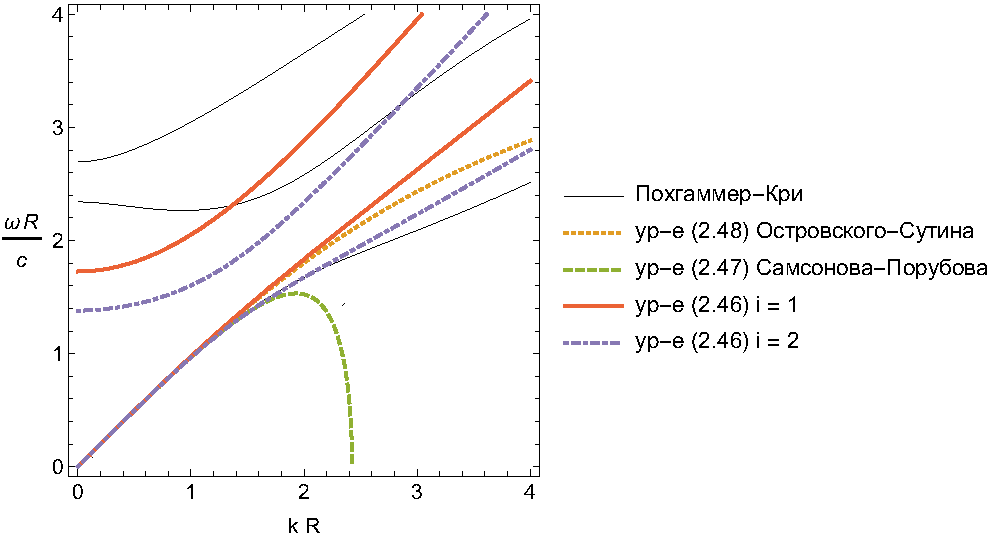
\includegraphics[width=0.85\linewidth]{Fig2}
	\caption{Дисперсионные кривые для стержня с $\nu = 0.34$. %сделанного из полистирола, упругие модули которого приведены в таблице~\ref{tab:ps}.
	}
	\label{fig:disp}
\end{figure} 

Все модели достаточно хорошо описывают нижнюю ветвь дисперсионной кривой в длинноволновой области, однако наиболее точной является модель (\ref{eq_dim_free_surf}, $i=2$). Уравнение Самсонова -- Порубова \eqref{eq_dim_SP} обладает коротковолновой неустойчивостью, в то время как остальные три модели не имеют такого эффекта. Отметим, что коротковолновая неустойчивость затрудняет численный счёт, поскольку высокочастотные гармоники в таком случае могут неограниченно возрастать. Полученные в настоящей работе уравнения \eqref{eq_dim_free_surf} в отличие от других уравнений улавливают вторую ветвь дисперсионной кривой, правда описывают её очень неточно: помимо большого отличия по значению, эти кривые имеют всюду положительный наклон, тогда как точная кривая имеет отрицательный наклон в области длинных волн, что соответствует отрицательной групповой скорости.
%Уравнение (\ref{eq_dim_free_surf}, $i=2$) лучше описывает нижнюю ветвь для коротких волн, в то время как (\ref{eq_dim_free_surf}, $i=1$) обладает лучшими дисперсионными свойствами как длинноволновая модель.

%Отметим, что улавливание ещё одной моды колебаний в численном моделировании является скорее недостатком, чем преимуществом, поскольку к длинным продольным волнам, для изучения которых была построена модель, подмешиваются другие колебания.
%All models reasonably well describe the lowest branch of the dispersion curves for the long waves. Eq. (\ref{eq_dim_SP})  suffers from a short-wave instability, while other three models do not have this defect. Eq. (\ref{eq_dim_free_surf}) for $i=1,2$, capture the presence of the second branch. We also note that, at least in this example, eq. (\ref{eq_dim_free_surf}) for $i=1$ has better dispersive properties than eq. (\ref{eq_dim_free_surf}) for $i=2$ (as a long-wave model). However, eq. (\ref{eq_dim_free_surf}) for $i=2$ better describes the lowest branch in the short wave region. 
%One can expect that both derived Boussinesq-type models in (\ref{eq_dim_free_surf}) can be useful, depending on the type of the dominant dispersive radiation in the problem under study. One could also try to artificially ``optimise" the dispersive properties as discussed, for example, in \cite{PAT, ADKM}. However, in this paper we were interested in the ``natural" derivation of Boussinesq-type models.

Все четыре уравнения (\ref{eq_dim_free_surf}, $i=1,2$), \eqref{eq_dim_SP} и \eqref{eq_dim_OS} имеют семейство солитонных решений:
\begin{equation}\label{soliton}
u_i(x,t) = A\ {\rm sech}^2\ \left[B_{i} \left(x\pm t \sqrt{c^2+\frac{A \beta_1}{3 \rho}}\right) \right], \quad i = \overline {1,4},
\end{equation}
где амплитуда $A$ является свободным параметром. Для заданной амплитуды $A$, соответствующие солитонные решения имеют одинаковую скорость, но разные параметры ширины $B_i$:
\begin{align}
%\label{B1}
%B_1 &=& \sqrt{\frac{3 A\beta c^2 \rho}{\left[18 c^4  \nu^2 \rho^2 + 6A\beta c^2  \nu^2  \rho - A^2 \beta^2 (\nu+1)\right] R^2}} \, ,\\
\label{Bi}
B_i &= \sqrt{\frac{3A\beta_1 E}{-4\left[(A\beta_1 + 3E)^2\alpha_1^{(i)} + 3E(A\beta_1 + 3E)\alpha_2^{(i)} + 9E^2\alpha_3^{(i)}\right] R^2}} \, , \quad i=1,2,\\
\label{B3}
B_3 &= \sqrt{\frac{A\beta_1}{\left[6\nu E + 2 A \beta_1 (\nu - 1)\right] \nu R^2}}\, , \\
\label{B4}
B_4 &= \sqrt{\frac{A\beta_1}{(6E + 2A\beta_1)\nu^2 R^2}},
\end{align}
для уравнений \eqref{eq_dim_free_surf}, \eqref{eq_dim_SP} и \eqref{eq_dim_OS} соответственно. Получению солитонных решений посвящено Приложение 2.

На рисунке \ref{fig:soliton} в левой части изображены четыре солитона, задаваемых формулами (\ref{soliton}) -- (\ref{B4}) и имеющих амплитудный параметр $A = -0.07$. Видно, что все четыре солитона имеют разную длину, причём <<регуляризованный>> солитон (\ref{B4}) самый длинный. Однако солитоны такой амплитуды вызывают напряжения близкие к пределу упругости для полистирола. В экспериментах с полистироловым стержнем, описанных в~\cite{Garbuzov}, амплитуда очень мала: $A \sim 10^{-3} - 10^{-4}$, следовательно, в главном порядке по $A$ во всех четырёх формулах параметр длины примерно равен
%In the left part of the Figure \ref{fig:soliton} we plot the four solitons given by the formulae (\ref{soliton}) - (\ref{B4}) for one and the same value of the amplitude parameter $A = -0.05$ and the same elastic moduli shown in Table \ref{tab:ps} (typical for a polystyrene \cite{HughesKelly}). We can see that the four solitons have a different width, with the regularised soliton (\ref{B4}) being the widest. However, this figure is plotted for the value of $A$ which exceeds the yield point for the polystyrene, and therefore in practice this difference would not be important for that particular material (but could be important for some other materials). Indeed, in experiments with polystyrene discussed in the next section the value of $A$ is very small, $A \sim 10^{-3} - 10^{-4}$. Therefore, to leading order in $A$, all four formulae will give the width parameter approximately equal to 
\begin{equation}\label{}
B = \sqrt{\frac{A\beta_1}{6\nu^2 E R^2}},
\end{equation}
а соответствующее солитонное решение изображено в правой части рисунка~\ref{fig:soliton} для $A = -0.001$.
\begin{figure}[h]
	\centering
	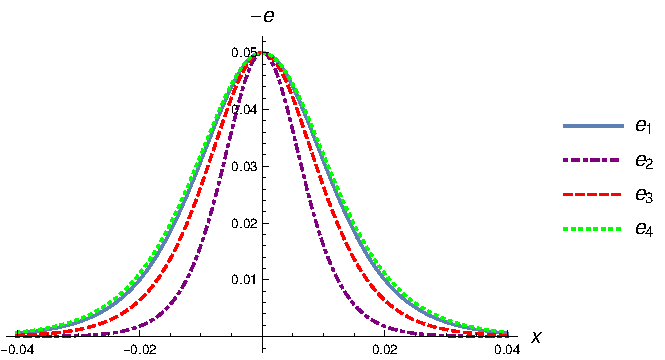
\includegraphics[width=0.54\linewidth]{Fig3a}
	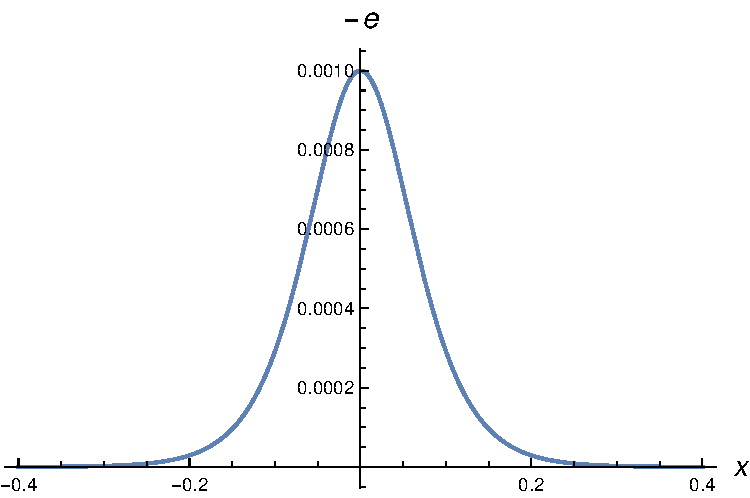
\includegraphics[width=0.42\linewidth]{Fig3b}
	\caption{Солитоны в стержне радиуса $R = 5$~мм, сделанном из полистирола при $A = -0.07$ (слева) и $A= -0.001$ (справа). Упругие модули полистирола приведены в таблице~\ref{tab:ps}.}
	\label{fig:soliton}
\end{figure}
\begin{table}[h]
	\begin{center}
		\begin{tabular}{|c|c|c|c|c|c|}
			\hline
			Модуль Юнга & Коэффициент & \multicolumn{3}{|c|} {Модули Мурнагана, Н/м\textsuperscript{2} } & Плотность \\
			\cline{3-5}
			$E$, Н/м\textsuperscript{2} & Пуассона, $\nu$ & $l$ & $m$ & $n$ & $\rho$, кг/м\textsuperscript{3}  \\
			\hline
			$3.7\cdot10^9$ & $0.34$ & $-18.9\cdot10^{9}$ & $-13.3\cdot10^{9}$ & $-10\cdot10^{9}$ & 1060 \\
			\hline
		\end{tabular}
	\end{center}
	\vspace{-5mm}
	\caption{Упругие модули полистирола~\cite{HughesKelly}.}
	\label{tab:ps}
\end{table}

На рисунке~\ref{fig:rod_deformed} показано, как выглядит деформированный стержень, когда по нему бежит солитон сжатия. Увеличенные перемещения позволяют увидеть эффект Пуассона (утолщение тела при продольном сжатии), а также нелинейную зависимость продольного перемещения от $r$ (вертикальные линии немного изгибаются в месте сжатия). На всякий случай напомним, что на рисунке~\ref{fig:soliton} изображён график продольной деформации на оси стержня, а не форма границы стержня на рисунке~\ref{fig:rod_deformed}. 
\begin{figure}[hh]
	\centering
	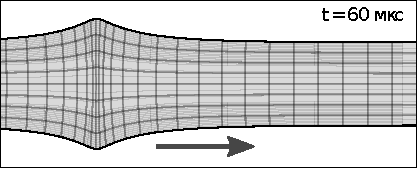
\includegraphics[width=0.6\linewidth]{DeformedRod1}
	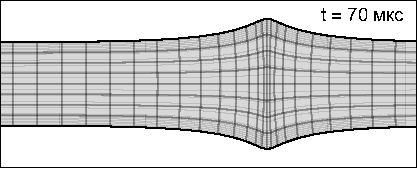
\includegraphics[width=0.6\linewidth]{DeformedRod2}
	\caption{Стержень из полистирола в разрезе при прохождении солитона деформации~\eqref{soliton},~\eqref{Bi} с амплитудным параметром $A=-0.03$. Продольные перемещения увеличены в 30 раз, поперечные в 60 раз.}
	\label{fig:rod_deformed}
\end{figure}

Репараметризуем солитонное решение \eqref{soliton} через скорость $v$ вместо амплитуды $A$:
\begin{align}
\label{soliton_v}
u_i(x, t) &= \frac{3 \rho \left(v^2 - c^2\right)}{\beta_1} {\rm sech}^{2}\left[\tilde{B_i}(x\pm v t)\right], \qquad v = \sqrt{c^2+\frac{A\beta_1}{3 \rho}} \, ,\\
\label{Bimod}
%\tilde{B}_1 &=& \sqrt{\frac{c^2(v^2- c^2)}{(2(\nu^2+\nu+1) c^2 v^2 - (\nu+1)(c^4+v^4))R^2}} \, ,\\
\tilde{B}_i &= \sqrt{\frac{c^2(v^2- c^2)}{-4\left(\alpha_1^{(i)} v^4 + \alpha_2^{(i)} c^2 v^2 + \alpha_3^{(i)}c^4\right)R^2}} \, , \quad i =1,2,\\
\label{B3mod}
\tilde{B}_3 &= \sqrt{\frac{v^2- c^2}{2\nu R^2 [c^2 - (1 - \nu) v^2 ]}} \, ,\\
\label{B4mod}
\tilde{B}_4 &= \sqrt{\frac{v^2- c^2}{2\nu^2 v^2 R^2}} \, .
\end{align}
%$$ B = \sqrt{\frac{3c^2(v^2- c^2)}{4((1+\nu+\nu^2) c^2 v^2 - (1+\nu)(c^4+v^4))H^2}} $$
%Regularized:
%\begin{equation}%\label{}
%u(x, t) = \frac{3 \left(v^2 - c^2\right)}{2\beta} \cosh^{-2}\left(\frac{1}{\nu v H}\sqrt{\frac{3(v^2- c^2)}{8}}(x\pm v t)\right),
%\end{equation}
Солитонное решение существует, только если параметр длины $\tilde{B}$ вещественен, и, следовательно, $\tilde{B}^2 > 0$, что приводит, предполагая $\nu < 0.5$, к следующим ограничениям на скорость солитона:
\begin{itemize}
	%\item $\tilde{B}_1^2 > 0 \implies$ $\displaystyle v^2 < \frac{(\nu^2 + \nu + 1) - \nu\sqrt{\nu^2 + 2\nu + 2}}{\nu + 1} c^2$ or $\displaystyle c^2 < v^2 < \frac{(\nu^2 + \nu + 1) + \nu\sqrt{\nu^2 + 2\nu + 2}}{\nu + 1} c^2$,
	\item $\tilde{B}_i^2 > 0 \implies$ $\displaystyle v^2 < \frac{-\alpha_2^{(i)} - \sqrt{\alpha_2^{(i)2} - 4\alpha_1^{(i)}\alpha_3^{(i)}}}{2\alpha_1^{(i)}} c^2$ или $\displaystyle c^2 < v^2 < \frac{-\alpha_2^{(i)} + \sqrt{\alpha_2^{(i)2} - 4\alpha_1^{(i)}\alpha_3^{(i)}}}{2\alpha_1^{(i)}} c^2$, $i=1,2$,
	\item $\tilde{B}_3^2 > 0 \implies$ $\displaystyle c^2 < v^2 < \frac{c^2}{1-\nu}$, 
	\item $\tilde{B}_4^2 > 0 \implies$ $c^2 < v^2$.
\end{itemize}
Отметим, что $\displaystyle 0 < \frac{-\alpha_2^{(i)} - \sqrt{\alpha_2^{(i)2} - 4\alpha_1^{(i)}\alpha_3^{(i)}}}{2\alpha_1^{(i)}} \leqslant 1$ и $\displaystyle \frac{-\alpha_2^{(i)} + \sqrt{\alpha_2^{(i)2} - 4\alpha_1^{(i)}\alpha_3^{(i)}}}{2\alpha_1^{(i)}} \geqslant 1$ $\forall \nu\in[0, 0.5]$ для $i=1,2$. 

Таким образом, в то время как первые три модели дают ограниченный диапазон скоростей солитона сжатия, регуляризованная модель не накладывает ограничения сверху на скорость. Также первые две модели, в отличие от двух других, допускают существование солитонов растяжения. 

Отметим, что помимо математического ограничения на параметры солитона (вещественность параметра ширины $B$) есть физическое ограничение: солитон не должен вызывать пластических деформаций, поскольку модель строилась только для упругих деформаций. Так, для полистирола и широкого круга других материалов именно физическое ограничение сильнее всего сужает диапазон допустимых скоростей, поскольку, как видно из формулы \eqref{soliton_v}, чем больше разность ${v^2-c^2}$, тем больше амплитуда и меньше длина солитона.
%Длинные волны в стержнях из таких материалов целесообразнее всего моделировать с помощью регуляризованной модели, являющейся наиболее простой среди рассмотренных моделей и в рамках которой не учитываются колебания других мод, а также отсутствует коротковолновая неустойчивость.

%Отметим, что все модели выведены в предположении малой амплитуды деформаций, которая пропорциональна относительной разнице $v^2$ и $c^2$. Однако все ограничения сверху на скорость солитона в стержне, например, из материала с $\nu\approx\frac13$ относительно далеки от $c^2$. Однако теоретически могут быть материалы с такими упругими характеристиками 
%Thus, while the first three model equations give a finite range for the speeds of compression solitary waves, the regularised model does not impose an upper bound (see also the related discussions in  \cite{S_book}). Also, the first two models allow for the existence of solitons of opposite polarity, while the other two models do not allow that.   It would be interesting to compare the predictions for the permissible range of soliton speeds and polarities with direct numerical simulations of the full problem formulation. This could guide some future laboratory experiments.


\chapter{Численное решение уравнений нелинейной теории упругости}
В главе 2 из полных нелинейных уравнений движения 
%\eqref{2_eq1_0}, \eqref{2_eq2_0} и граничных условий \eqref{2_bc_rr}, \eqref{2_bc_rx} 
выведены упрощённые модели типа Буссинеска, описывающие длинные продольные волны деформации, которые теперь интересно сравнить с численным решением полных уравнений.

В настоящей работе основной интерес представляют непрерывные гладкие решения нелинейных уравнений. Наилучшим средством для этого является псевдоспектральный метод, с помощью которого мы будем решать как пространственно одномерные уравнения типа Буссинеска, так и полные трёхмерные уравнения движения.
Отметим, что пседвоспектральный метод чаще всего используется только для пространственной дискретизации, в то время как дискретизация по времени осуществляется с помощью стандартных методов, например, Рунге-Кутты 4-го порядка.
%Опишем метод подробнее.

Семейство спектральных методов, одним из которых является псевдоспектральный метод или метод коллокации, основано на поиске решения задачи в некотором подпространстве, имеющем конечный базис, в качестве которого чаще всего выбирается базис Фурье (набор синусов и косинусов) или семейство ортогональных многочленов. 
%Выбор базиса определяется граничными условиями Дирихле: базисные функции должны удовлетворять им. 
%Псевдоспектральный метод, называемый также методом коллокации, является одним из семейства спектральных методов. 
Отличительной особенностью псевдоспектрального метода является выполнение уравнений не на всей области, а лишь в конечном наборе точек, называемых точками коллокации. Получаемые в результате значения решения в точках коллокации затем интерполируются на всю область задачи. 
%В качестве точек коллокации выбираются точки соответствущей квадратуры, что определяется нулями определённых полиномов.
%Конкретный вид полинома, у которого ищутся нули, определяется типом квадратуры (Гаусса, Радау, Гаусса-Лобатто).
%При этом нули полиномов Чебышева и их производных имеют простой аналитический вид. А вот для полиномов Лежандра все сложнее и нули надо искать численно.
Выбор точек коллокации определяется используемым базисом: для базиса Фурье точки равномерно распределены по области, а для ортогональных многочленов выбираются точки соответствующей квадратуры, задаваемые нулями определённых многочленов. Конкретный вид многочлена, у которого ищутся нули, определяется типом квадратуры: Гаусса, Гаусса-Радо или Гаусса-Лобатто. Более подробному описанию этого метода применительно к решаемым уравнениям посвящён следующий параграф.

%Выбор этих точек определяется используемым базисом: для базиса Фурье точки равномерно распределены по области, а для многочленов Чебышёва эти точки должны быть распределены согласно чебышёвской плотности с разрежением в центре области и сгущением к краям. Неправильный выбор точек коллокации грозит возникновением больших ошибок в решении.

\section{Численная схема}
\subsection{Одномерное уравнение типа Буссинеска}
Сформулируем задачу Коши для одномерного регуляризованного уравнения Буссинеска с внешним воздействием:
\begin{align}
\label{3_bq_reg}
\begin{split}
&u_{tt} - c^2 u_{xx} - g_1 P_{xx} - g_2 T_x - \left(\tilde{\beta}_1 u^2 + \tilde{\beta}_2 u P + \tilde{\beta}_3 P^2\right)_{xx} + \tilde\alpha u_{xxtt}\\
&\qquad\qquad\qquad\qquad\qquad + \gamma_1 P_{xxxx} + \gamma_2 P_{xxtt} +\gamma_3 T_{xtt} + \gamma_4 T_{xxx} = 0, \quad x\in(0, L),
\end{split}\\
\label{3_bq_iv}
&u(x, 0) = \phi(x), \qquad u_t(x, 0) = \psi(x),%\\
%\label{3_bq_bc}
%&u(0, t) = u(L, t).
\end{align}
где на границах области поставлены условия симметрии, поскольку модель Буссинеска выводилась для бесконечного стержня. Уравнение \eqref{3_bq_reg} совпадает по форме с \eqref{2_eq_fin_reg}, где некоторые коэффициенты переобозначены для лаконичности записи.

Будем решать регуляризованное уравнение типа Буссинеска с помощью псевдоспектрального метода Фурье. Для этого сначала отобразим область задачи $(0, L)$ в $(0, 2\pi)$ с помощью замены $\tilde x = Sx$, где $S = 2\pi/L$, и запишем новое уравнение, опустив тильду над $x$:
\begin{equation}
\label{3_bq_reg_scaled}
\begin{split}
&u_{tt} - S^2 c^2 u_{xx} - S^2 g_1 P_{xx} - S g_2 T_x - S^2\left(\tilde{\beta}_1 u^2 + \tilde{\beta}_2 u P + \tilde{\beta}_3 P^2\right)_{xx} + S^2\tilde\alpha u_{xxtt}\\
&\qquad\qquad\qquad\qquad + S^4\gamma_1 P_{xxxx} + S^2\gamma_2 P_{xxtt} + S\gamma_3 T_{xtt} + S^3\gamma_4 T_{xxx} = 0, \quad x\in(0, 2\pi),
\end{split}
\end{equation}
Будем искать приближённое решение $u_N$ в виде комбинации из $N$ гармоник:
\begin{equation}\label{3_spect_approx}
u_N(x, t) = \sum_{k=-N/2}^{N/2-1} \widehat u(k, t) e^{ikx}, \quad x\in(0, 2\pi).
\end{equation}
Ключевая идея псевдоспектрального метода заключается в поиске таких коэффициентов $\widehat u(k, t)$, что точное решение $u$ совпадает с приближённым решением $u_N$ в точках коллокации $x_j$:
\begin{equation}\label{3_pseudo_sp_approx}
u_N(x_j, t) = u(x_j, t), \quad x_j = \frac{2\pi j}{N}, \quad j=0,\dots, N-1.
\end{equation}
Из условия \eqref{3_pseudo_sp_approx} естественным образом вытекает применение дискретного преобразования Фурье (ДПФ) для нахождения $\widehat u(k, t)$, а для обратной операции -- обратного ДПФ:
%Для нахождения коэффициентов $\widehat u(k, t)$ при гармониках по значениям в узлах сетки используется дискретное преобразование Фурье (ДПФ), а для обратной операции -- обратное ДПФ:
\begin{align}\label{3_dft}
\widehat u(k, t) &= \mathcal{F} u = \frac1N\sum_{j=0}^{N-1} u(x_j, t) e^{-ikx_j}, \quad k=-\frac N 2, \dots, \frac N 2 - 1,\\
\label{3_idft}
u(x_j, t) &= \mathcal{F}^{-1} \widehat u = \sum_{k=-N/2}^{N/2-1} \widehat u(k, t) e^{ikx_j}, \quad j=0, \dots, N-1.
\end{align}
Отметим, что использование ДПФ выгодно с вычислительной точки зрения, поскольку для его реализации есть алгоритм быстрого преобразования Фурье.

Спектральное представление \eqref{3_spect_approx} позволяет быстро находить производную по пространственной переменной:
\begin{equation}\label{3_spect_deriv}
u_N'(x, t) = \sum_{k=-N/2}^{N/2-1} ik \widehat u(k, t) e^{ikx}.
\end{equation}
Применим спектральное представление \eqref{3_spect_approx} к уравнению \eqref{3_bq_reg_scaled} и начальным условиям \eqref{3_bq_iv}. Приравнивая коэффициент при каждой гармонике к нулю, получаем систему обыкновенных дифференциальных уравнений с начальными условиями в виде:
\begin{gather}\label{3_bq_reg_dft}
\begin{split}
\lb 1 - \tilde{\alpha} S^2 k^2\rb\ddot{\widehat u} =&  -S^2 k^2 \lb c^2 \widehat u + \tilde \beta_1 \widehat{u^2} + \tilde\beta_2\widehat{uP} + \tilde{\beta}_3\widehat{P^2} \rb + S^2 g_1 \widehat{P_{xx}} - S g_2 \widehat{T_x} \\
&- \lb S^4\gamma_1 \widehat{P_{xxxx}} + S^2\gamma_2 \widehat{P_{xxtt}} + S\gamma_3 \widehat{T_{xtt}} + S^3\gamma_4 \widehat{T_{xxx}}\rb,
\end{split}\\
\label{3_bq_dft_iv}
\widehat{u}(k, 0) = \widehat{\phi}(k), \qquad \dot{\widehat{u}}(k, 0) = \widehat{\psi}(k), \qquad k=-\frac N 2, \dots, \frac N 2 - 1,
\end{gather}
где точка над функцией обозначает производную по времени.
Для нахождения Фурье образа нелинейного слагаемого $u^2$, а также $uP$, к функции $\widehat u$ применяется обратное преобразование, затем полученная функция $u(x_j, t)$ возводится в квадрат в узлах сетки или домножается на $P(x_j, t)$ и переводится обратно в пространство Фурье:
$$
\widehat{u^2} = \mathcal{F}\lbrack\lb\mathcal{F}^{-1}\widehat u\rb^2\rbrack, \qquad \widehat{uP} = \mathcal{F}\lbrack P\cdot \mathcal{F}^{-1}\widehat u\rbrack.
$$
Такой метод при использовании быстрого преобразования Фурье позволяет эффективно вычислять $\widehat{u^2}$ и $\widehat{uP}$.
Решать систему \eqref{3_bq_reg_dft}, \eqref{3_bq_dft_iv} будем с помощью метода Рунге-Кутты 4-го порядка. Применяя обратное ДПФ к решению этой системы, получаем приближение исходной задачи Коши \eqref{3_bq_reg}, \eqref{3_bq_iv}.

С помощью псевдоспектрального метода уравнения в частных производных часто сводятся к системе ОДУ относительно значений функции в точках коллокации $u_N(x_j, t)$, а не $\widehat u(k, t)$. В таком случае нелинейные слагаемые вычисляются простым поточечным произведением значений функций в точках коллокации, а вычисление пространственных производных осуществляется с помощью ДПФ и формулы ~\eqref{3_spect_deriv}. Отметим, что вычисление производной может быть выражено через умножение вектора значений $u_N(x_j, t)$ на матрицу производной $D_N$:
\begin{equation}\label{3_phys_deriv}
\vect{u}_N'(t) = D_N \vect{u}_N(t), \qquad \vect{u}_N(t) = \{u_N(x_j, t)\}_{j=0}^{N-1}.
\end{equation}
Однако для регуляризованного уравнения Буссинеска, где присутствует смешанная производная $u_{xxtt}$, применить такой метод вычисления производной затруднительно. Матрицы $D_N$ для различных базисов приведены в~\cite{Canuto2007}.
%Для базиса Фурье она записывается следующим образом:
%\begin{equation}\label{3_diff_mat_fourier}
%(D_N)_{jl} = \begin{cases}
%\frac12(-1)^{j+l} \ctg\lbrack\frac{(j-l)\pi}{N}\rbrack, &j\neq l,\\
%0, &j=l,
%\end{cases}
%\end{equation}
%а для базиса Лежанжра в точках Гаусса-Лобатто и Гаусса-Радо так:
%\begin{equation}\label{3_diff_mat_legendre}
%(D_N)_{jl} = \begin{cases}
%\dfrac{L_N(x_j)}{L_N(x_l)} \dfrac{1}{x_j-x_l}, &j\neq l,\\
%-\dfrac{(N+1)N}{4}, &j=l=0,\\
%\dfrac{(N+1)N}{4}, &j=l=N,\\
%0, &\mbox{в остальных случаях},
%\end{cases}
%\end{equation}

Аналогичным образом можно дискретизировать нерегуляризованные уравнения (\ref{eq_dim}) с тремя дисперсионными слагаемыми, однако возникающая система обыкновенных дифференциальных уравнений 4-го порядка оказывается жёсткой и не поддаётся решению явными методами. В настоящей работе много времени было уделено реализации псевдоспектрального метода для полных уравнений, описанию которого посвящён следующий пункт, поэтому задачу о численном моделировании уравнений \eqref{eq_dim} было решено оставить на будущее.

\subsection{Полные трёхмерные уравнения}
%Разрабатывая численный метод для решения полных уравнений, мы задались целью сделать его пригодным для как можно более широкого круга численных экспериментов. Во-первых, метод должен подходить для моделирования эволюции некоторого начального импульса в течение длительного времени, для чего необходимо иметь возможность задачу Коши на периодическом интервале. Во-вторых, метод должен позволять моделировать волны, возникающие в результате внешнего воздействия, как на боковую поверхность, так и на торец стержня (решение начально-краевой задачи на некотором конечном, но достаточно длинном интервале). %В третьих, мы хотели бы учитывать в будущем не только осесимметричную деформацию, т.е. случай, когда перемещение зависит от угловой координаты $\varphi$.

%Для того, чтобы выполнить поставленные цели, мы реализовали метод с дискретизацией по всем трём координатам. Для возможности моделирования уравнений в длинных стержнях с высокой точностью без рассмотрения гармоник или полиномов большой степени, мы реализовали многодоменный метод, позволяющий разбить область по осевой координате на несколько подобластей (доменов). Например, если нужно иметь 1000 точек коллокации по оси $x$, то, чтобы избежать учёт полиномов 1000-й степени, можно разбить область на 50 подобластей и на каждой подобласти использовать полиномы до 20-й степени. {\color{red} Поправить вводную часть после описания экспериментов}

Сформулируем задачу Коши для полных уравнений, описывающих динамику однородного стержня круглого сечения длиной $L$ и радиусом $R$:
\begin{align}
\label{3_eqns_full}
&\ddot{\vect{U}}(x, r, \varphi, t) = \frac1\rho \nabla\cdot\tens{P},\quad 0<x<L, \quad 0<r<R,\quad 0<\varphi<2\pi,\\
\label{3_bc_full}
&\tens{P} \cdot \vect{n} = \vect{P_b}, \quad r = R,\\
\label{3_iv_full}
&\vect{U}(x,r,\varphi,0) = \vect{U}_0(x,r,\varphi), \quad \vect{\dot U}(x,r,\varphi,0) = \vect{\dot U}_0(x,r,\varphi),\\
\label{3_stress}
&\tens{P} = \lambda \lb\trace{\tens{E}}\rb \tens{\mathcal{I}} + 2\mu \tens{E} + l \lb\trace{\tens{E}}\rb^2 \tens{\mathcal{I}} - m\lb \lb\trace{\tens{E}}\rb^2\tens{\mathcal{I}} - 2\lb\trace{\tens{E}}\rb\tens{E} - \lb\trace{\tens{E}^2}\rb\tens{\mathcal{I}}\rb + n\lb\tens{E}^*\rb^T,\\
\label{3_strain}
&\tens{E} = \frac12 \lb \nabla\vect{U}^T + \nabla\vect{U} + \nabla\vect{U}^T \cdot \nabla\vect{U} \rb,
\end{align}
где $\tens{E}^*$ -- союзная матрица, $\tens{\mathcal{I}}$ -- единичный тензор, а по $x$ ставятся периодические граничные условия.
Будем искать решение в некотором конечномерном пространстве, задаваемым системой базисных функций $\Phi_{n_1}(x)$, $\Psi_{n_2}(r)$, $\Theta_{n_3}(\varphi)$. 
Представим приближённое решение %на $i$-м домене
$\vect{U}_{N}$ в спектральном виде и потребуем, чтобы приближённое решение совпадало с точным в точках коллокации:
\begin{align}
\label{3_spect_approx_full}
&\vect{U}_{N}(x,r,\varphi,t) = \sum_{n_1,n_2,n_3} \vect{\widehat{U}}(n_1,n_2,n_3,t) \Phi_{n_1}(x) \Psi_{n_2}(r) \Theta_{n_3}(\varphi),\\
\label{3_pseudo_sp_approx_full}
\begin{split}
&\vect{U}_{N}(x_{j_1}, r_{j_2}, \varphi_{j_3}, t) = \vect{U}(x_{j_1}, r_{j_2}, \varphi_{j_3}, t), \quad j_1 = 0,\dots, N_1-1, \quad j_2 = 0,\dots, N_2-1,\\
&\hspace{72.5mm} j_3 = 0,\dots, N_3-1.
\end{split}
\end{align}
В уравнении \eqref{3_eqns_full} отсутствуют смешанные производные по временной и пространственным переменным, поэтому подстановка \eqref{3_spect_approx_full} в \eqref{3_eqns_full} приводит к системе ОДУ второго порядка относительно~$\vect{U}$:
\begin{equation}\label{3_ode_inner}
\vect{\ddot{U}}_{N,k} = F_{k}(\vect{U}_{N,k_0}, \dots, \vect{U}_{N,k_N}), \quad k = k_0, \dots, k_N.
\end{equation}
Здесь $k$ -- мультииндекс: $k = (j_1,j_2,j_3)$, $k_0=(0,0,0)$, $k_N = (N_1-1,N_2-1,N_3-1)$, а также использовано обозначение: $\vect{\widehat U}_{N,j_1,j_2,j_3} = \vect{\widehat U}_{N}(x_{j_1}, r_{j_2}, \varphi_{j_3}, t)$. В граничных узлах необходимо сделать добавку, чтобы выполнялись граничные условия \eqref{3_bc_full}:
\begin{equation}\label{3_ode_boundary}
\vect{\ddot{U}}_{N,k} = F_{k}(\vect{U}_{N,k_0}, \dots, \vect{U}_{N,k_N}) + \vect{P}_{b,k} - \vect{P}(\vect{U}_{N,k_0}, \dots, \vect{U}_{N,k_N}), \quad r_k = R.
\end{equation}

Функция $F_k$ содержит в себе множество пространственных производных, которые можно вычислить по формуле~\eqref{3_phys_deriv} с помощью умножения на матрицу дифференцирования $D_N$. Оценим сложность этого метода на примере вычисления спектральной производной:
\begin{align} \label{3_spect_deriv_example}
&\lb\pdiff{U_N}{x}\rb_{j_1, j_2, j_3} = \lb D_{N_1}\rb_{j_1 l} U_{N,l,j_2,j_3},
\begin{split} 
j_1 = 0,\dots, N_1-1, \quad &j_2 = 0,\dots, N_2-1,\\
&j_3 = 0,\dots, N_3-1,
\end{split}
\end{align}
где в правой части выполняется суммирование по повторяющемуся индексу $l$. Такое вычисление производной требует $O(N_1^2N_2N_3)$ операций. Если в задаче используется базис Фурье или Чебышёва, то дифференцирование можно провести в пространстве коэффициентов $\widehat{U}_N$, для перехода к которым используется быстрое преобразование Фурье, что потребует $O\lb N_1\log(N_1) N_2 N_3\rb$ операций. Если используется другой базис, например, Лежандра, то такой возможности ускорить вычисление производной нет.

Для того, чтобы справиться с этой проблемой и иметь возможность относительно быстро получать решения уравнений на сетке с большим количеством точек, мы применили \emph{многодоменный} псевдоспектральный метод, он же метод \emph{спектрального элемента}.
В рамках этого метода область задачи $\Omega$ разбивается по каждой из осей на $M$ подобластей (доменов) $\Omega_m$:
\begin{align*}
&\Omega = \{(x,r,\varphi)\in\mathbb{R}^3 \, | \, 0<x<L, \; 0<r<R, \; 0<\varphi<2\pi\} = \bigcup\limits_{i=1}^{M} \Omega_m,\\
&\Omega_m = \{(x,r,\varphi)\in\mathbb{R}^3 \, | \, 0\leqslant L_{m}<x<L_{m+1}\leqslant L, \; 0<R_m<r<R_{m+1}\leqslant R, \\
&\hspace{40mm} 0\leqslant \varphi_m<\varphi<\varphi_{m+1}\leqslant 2\pi\}.
\end{align*}
На каждом домене осуществляется дискретизация согласно псевдоспектральному методу, а затем домены сшиваются так, как это происходит в методе конечных элементов. Теперь для вычисления производной \eqref{3_spect_deriv_example} требуется $O(M N_{1,M}^2 N_{2,M} N_{3,M})$, где $N_{1,M}$, $N_{2,M}$, $N_{3,M}$ --- размерность базиса на одном домене. Выбирая базисы не слишком большой размерности на каждом элементе, мы сможем добиться более высокой скорости вычисления пространственных производных.
%Отметим, что если на доменах выбирать базисы небольшой размерности, то вычисление производной с помощью умножения на матрицу дифференцирования будет происходить быстрее, чем с помощью быстрого преобразования Фурье, за счёт меньшей константы.
%Отметим, что для реализации периодических условий по $x$, 

В настоящей работе представляют интерес решения уравнений в осесимметричном случае, поэтому дискретизацию по $\varphi$ в численных экспериментах, описанных в следующем параграфе, мы не будем.
Для дискретизации по $x$ и по $r$ мы будем использовать базис Лежандра, причём по $x$ в качестве точек коллокации выбираются точки Гаусса-Лобатто, включающие границы, а по $r$ --- точки Гаусса-Радо, чтобы исключить центральную точку стержня ($r=0$). 

%Система ОДУ \eqref{3_ode_inner}, \eqref{3_ode_boundary} была получена путём вычисления пространственных производных в \eqref{3_eqns_full}, \eqref{3_bc_full}, \eqref{3_strain} с помощью умножения на матрицу дифференцирования, как в~\eqref{3_phys_deriv}. Однако умножение массива значений функции на матрицу --- дорогостоящая операция. Например, для вычисления $\pdiff{U}{x}$ необходимо умножить массив значений $\{U_N\}_{k=k_0}^{k_N}$ размером $N_1\times N_2\times N_3$ на матрицу дифференцирования $D_N$ размером $N_1\times N_1$, что требует $O(N_1^2N_2N_3)$ операций.

%Следующая задача -- сшивка доменов -- проводится также, как в методе конечных элементов. 
%\begin{figure}[h]
%	\centering
%	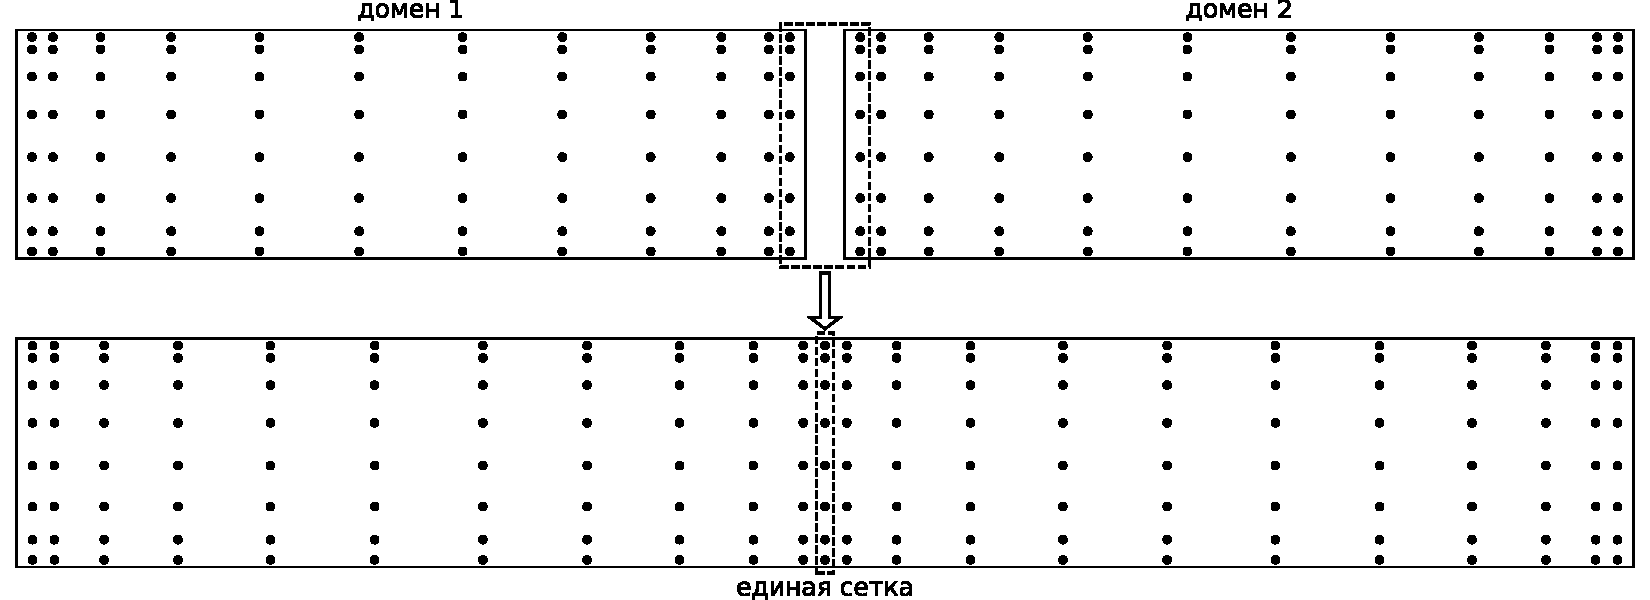
\includegraphics[width=\linewidth]{figures/DomainConnect}
%	\caption{Сшивка доменов.}
%	\label{fig:domain_connect}
%\end{figure}



\section{Численные эксперименты}

\subsection{Образование солитона из начального условия}
Будем решать задачу Коши для полных уравнений, где начальное условие задано распространяющимся вправо со скоростью $c$ гладким импульсом:
\begin{flalign}
\label{3_ic_u}
&\qquad U_0 (x, r) = A_0 W \erf\lb \frac{x - L/2}{W}\rb,&  &\dot{U}_0 (x, r) = -c \pdiff{U_0}{x}&\\
\label{3_ic_v}
&\qquad V_0(x, r) = -\nu r \pdiff{U_0}{x},& &\dot{V}_0 (x, r) = -c \pdiff{V_0}{x}&
\end{flalign}
На рисунке~\ref{fig:evol_compar1} слева изображена эволюция этого импульса и зарождение солитона при $A_0=0.01$, $W=20$ в стержне из полистирола, характеристики которого представлены в таблице~\ref{tab:ps}. Исходный импульс испускает некоторые осцилляции и отрывается от них, что согласуется с моделью Буссинеска, согласно которой солитон имеет большую скорость, чем линейные волны. На рисунке справа представлено сравнение оторвавшегося импульса (<<экспериментального>> солитона) с <<теоретическим>> солитонном \eqref{soliton_v}. Если скорость теоретического солитона, являющуюся свободным параметром в \eqref{soliton_v}, подобрать так, чтобы она совпадала со скоростью экспериментального солитона, то последний имеет почти ту же длину, что и теоретический, но на 6\% большую амплитуду.
\begin{figure}[h]
	\centering
	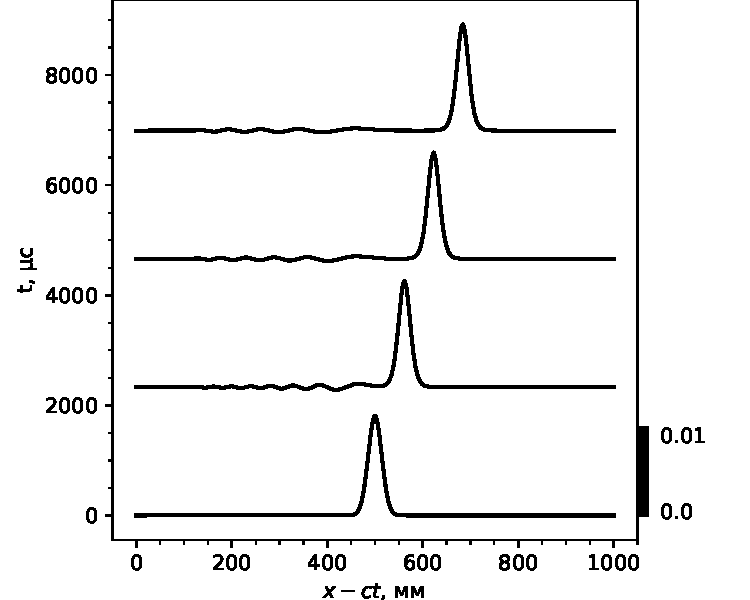
\includegraphics[width=0.49\linewidth]{figures/SolEvol}
	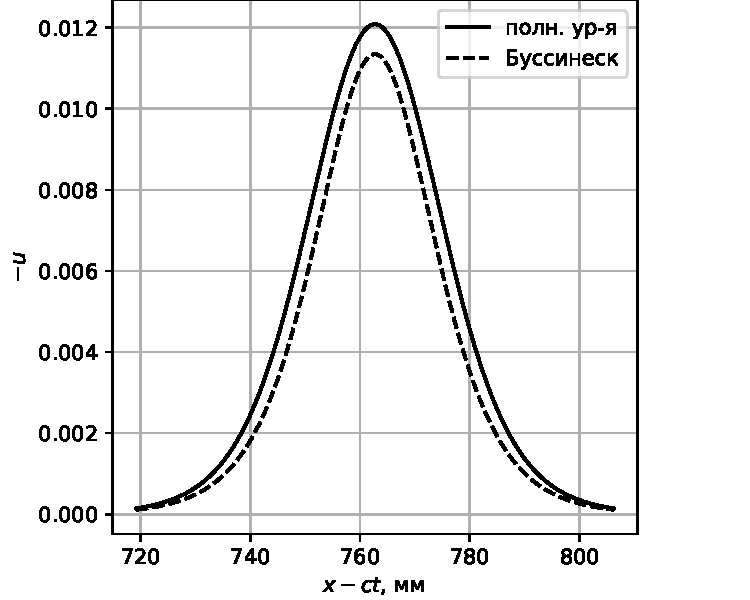
\includegraphics[width=0.49\linewidth]{figures/SolCompare}
	\caption{Слева: решение задачи Коши с начальными условиями \eqref{3_ic_u}, \eqref{3_ic_v} для полных уравнений. На графике изображены профили продольной деформации в центре стержня ($r=0$) в различные моменты времени:~$-U_x(x - ct, 0, t)$. Масштаб деформации показан чёрным прямоугольником. Справа: сравнение профиля <<экспериментального>> солитона, полученного в численном эксперименте, и <<теоретического>> солитона \eqref{soliton_v}. Скорость теоретического солитона $v$ подобрана так, чтобы она совпадала со скоростью экспериментального.}
	\label{fig:evol_compar1}
\end{figure}

Теперь решим аналогичную задачу Коши для регуляризованного уравнения типа Буссинеска, где начальное условие задано формулой:
\begin{flalign}
\label{3_bq_ic}
&\qquad u_0 (x) = 2A_0 \exp\lb \frac{(x - L/2)^2}{W^2}\rb,&  &\dot{u}_0 (x) = -c \pdiff{u_0}{x}.&
\end{flalign}
Отметим, что уравнение Буссинеска записано относительно функции $u = U_{x}$, а выражение поперечного перемещения $V$ через продольное $U$ уже <<вшито>> в модель.
На рисунке~\ref{fig:evol_compar2} слева представлено сравнение эволюции импульса согласно полным уравнениям и согласно модели Буссинеска.
Обе модели показывают качественно одинаковый результат, однако модель Буссинеска в этом эксперименте дала солитон примерно на 8\% большей амплитуды и, как следствие, бегущий быстрее солитона в полной модели.
\begin{figure}[h]
	\centering
	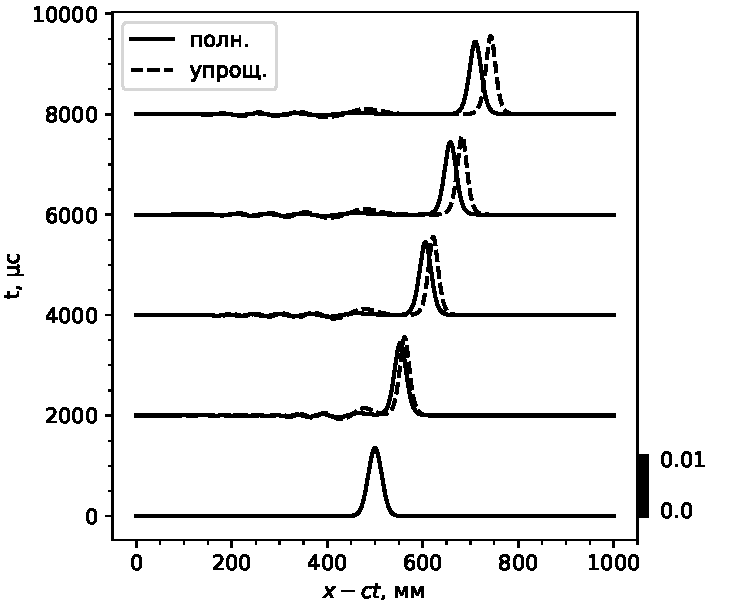
\includegraphics[width=0.49\linewidth]{figures/SolEvolCompare}
	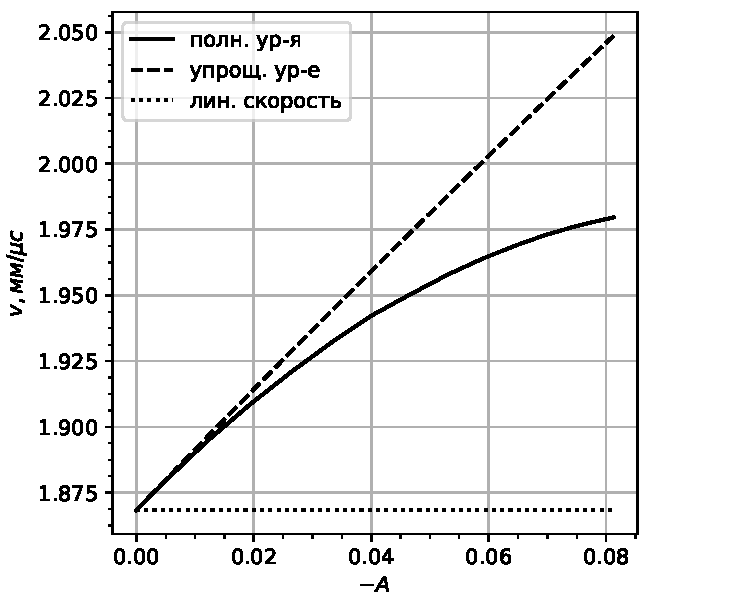
\includegraphics[width=0.49\linewidth]{figures/VelAmpl}
	\caption{Слева: сравнение решения задачи Коши~\eqref{3_ic_u}, \eqref{3_ic_v} для полной модели и задачи Коши~\eqref{3_bq_ic} для регуляризованной модели Буссинеска. Справа: сравнение <<экспериментальной>> и <<теоретической>> зависимостей скорости от амплитуды. Горизонтальная линия -- скорость линейных продольных волн $c$.}
	\label{fig:evol_compar2}
\end{figure}

Отличительной особенностью нелинейных волн является зависимость скорости от амплитуды волны. На основе численных решений задачи Коши для полных уравнений с начальными импульсами разной амплитуды можно построить <<экспериментальную>> зависимость скорости от амплитуды образовавшегося солитона и сравнить её с <<теоретической>>, задаваемой формулой \eqref{soliton_v}. Эти зависимости изображены на рисунке \ref{fig:evol_compar2} справа. Теоретическая зависимость для небольших амплитуд почти линейна, в то время как в численном эксперименте рост скорости солитона существенно замедляется с увеличением амплитуды.
%\begin{figure}
%	\centering
%	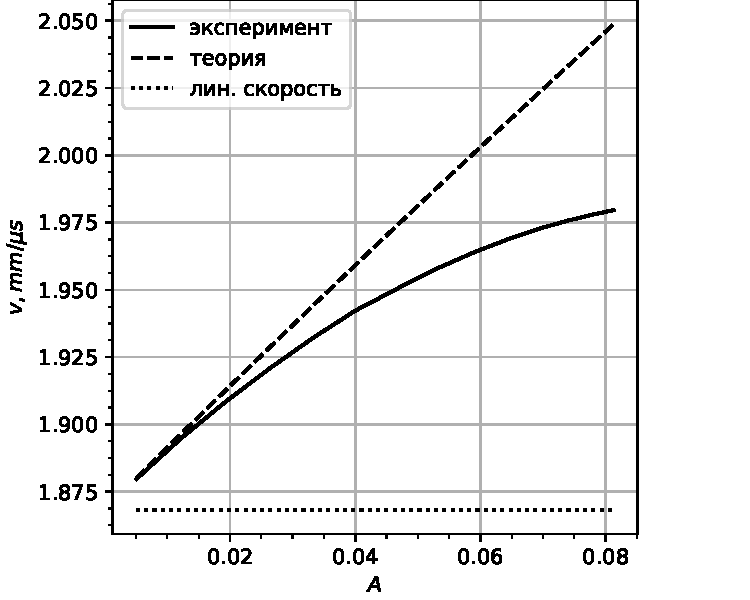
\includegraphics[width=0.6\linewidth]{figures/vel_ampl}
%	\caption{Сравнение <<экспериментальной>> и <<теоретической>> зависимостей скорости от амплитуды. Горизонтальная линия -- скорость линейных продольных волн $c$.}
%	\label{fig:vel_ampl}
%\end{figure}


\subsection{Образование солитона из бегущего по поверхности напряжения}
Выведенная модель типа Буссинеска отличается от полученных ранее учётом напряжения на поверхности. 
\begin{figure}[h]
	\centering
	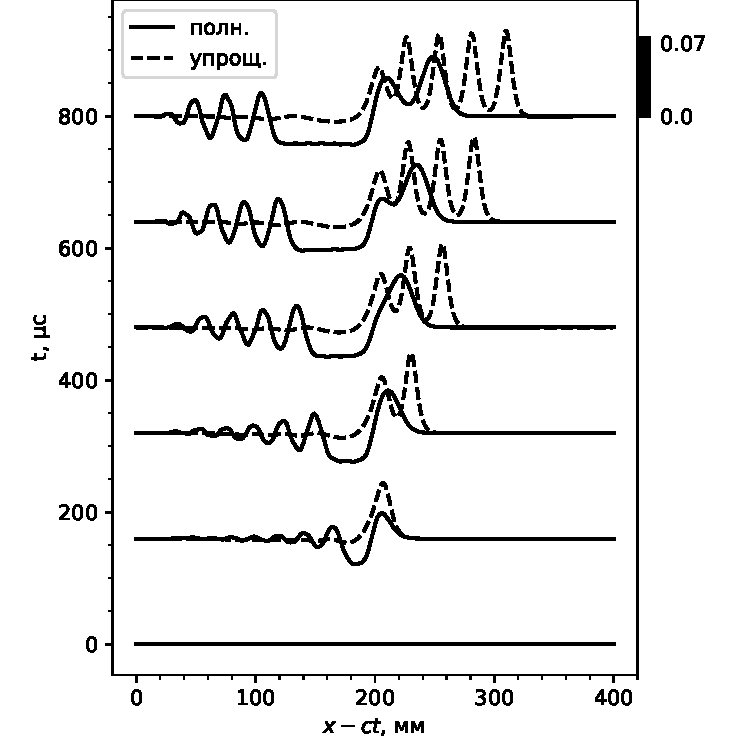
\includegraphics[width=0.49\linewidth]{figures/SolGenForceCompare}
	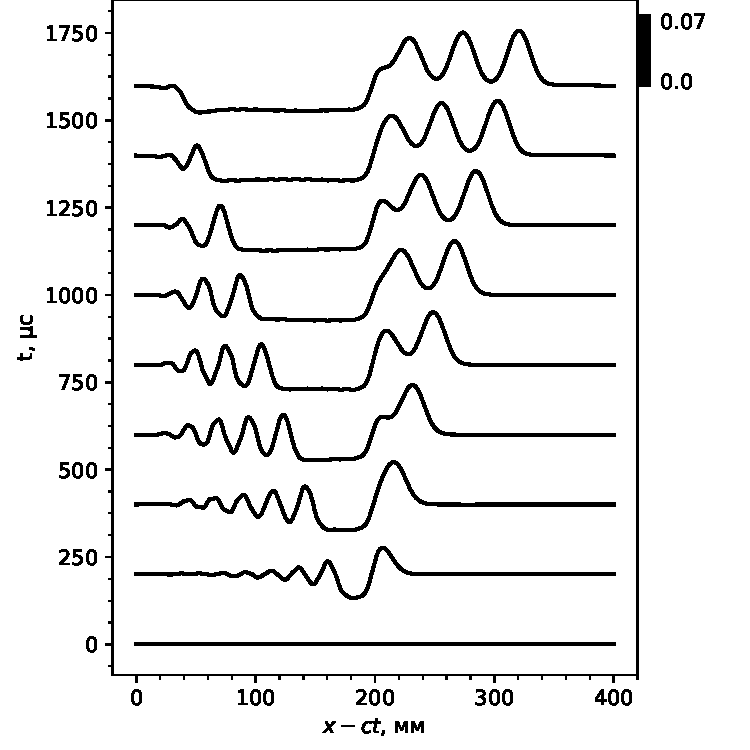
\includegraphics[width=0.49\linewidth]{figures/SolGenForce}
	\caption{}
	\label{fig:gen_compar1}
\end{figure}


\subsection{Образование солитона из удара по торцу стержня}
В предыдущем параграфе моделирование волн проводилось в стержне со свободной от напряжений поверхностью, однако представляет интерес изучение волн, вызываемых внешним воздействием, например, ударом по торцу стержня. Эти результаты могут быть полезны для того, чтобы возбудить уединённые волны в эксперименте. 

Модель типа Буссинеска строилась для бесконечного стержня, следовательно, она применима для описания волн вдали от торцов стержня. Моделирование волн вблизи торцов возможно с помощью полных уравнений движения. На рис. ... представлены результаты 

%\chapter{Обработка экспериментальных данных}


\chapter*{Заключение}
\addcontentsline{toc}{chapter}{Заключение}


\begin{thebibliography}{99}
	\addcontentsline{toc}{chapter}{Список источников}
	% Nonlinear waves: history review and general books 
	\bibitem{Dodd} Додд Р., Эйлбек Дж., Гиббон Дж., Моррис Х. Солитоны и нелинейные волновые уравнения. М.: «Мир», 1988.
	%\bibitem{Ablowitz} Абловиц М., Сигур Х. Солитоны и метод обратной задачи. М.: Мир, 1987.
	\bibitem{Ablowitz2011} M.J. Ablowitz, \textit{Nonlinear dispersive waves: asymptotic analysis and solitons}, Cambridge University Press, Cambridge, 2011.
	%\bibitem{Russel} Scott Russell J. \textit{Report on waves}, Rept. 14th meetings of the British Assoc. for the Advancement of Science. London: John Murray, 1844. P. 311–390.
	%\bibitem{Boussinesq} Boussinesq J. The?orie de l’intumescence liquid apple?e onde solitarie ou de translation se propagent dans un canal rectangularie // Comptes Rendus. 1871. Vol. 72. P. 755–759.
	%\bibitem{Korteweg} Korteweg D.J., de Vries G. On the change of form of long waves advancing in a rectangular channel, and on a new type of long stationary waves // Phil. Mag. 1895. Vol. 39. P. 422–443.
	%\bibitem{BBM} T.B. Benjamin, J.L. Bona, and J.J. Mahony, Model equations for long waves in nonlinear dispersive systems, \textit{Philos. Trans. R. Soc. London, Ser. A} 272(1220) (1972) 47-78.
	\bibitem{Zabusky} Zabusky N.J., Kruskal M.D. Interaction of «solitons» in a collisionless plasma and the reccurence of initial states // Phys. Rev. Lett. 1965.	Vol. 15, No 6. P. 240–243.
	\bibitem{GardnerIST} Gardner C.\,S., Greene J.\,M., Kruskal M.\,D., Miura R.\,M., Method for Solving the Korteweg-de Vries Equation, Physical Review Letters, 1967, 19(19), 1095--1097.
	\bibitem{Zakharov} Захаров В.\,Е., Манаков С.\,В., Новиков С.\,П., Питаевский Л.\,П., Теория солитонов: метод обратной задачи, Наука, М., 1980. 
	
	% Numerical methods review
	\bibitem{Taha} Taha T.\,R., Ablowitz M.\,I., Analytical and numerical aspects of certain nonlinear evolution equations. III. Numerical, Korteweg-de Vries equation, Journal of Computational Physics, 1984, 55(2), 231--253.
	\bibitem{Christov} Christov C.\,I., Conservative Difference Scheme for Boussinesq Model of Surface Waves, Proceedings ICFD 5, 1996, 343--349.
	\bibitem{Kolkovska} Kolkovska N., Dimova M., A new conservative finite difference scheme for Boussinesq paradigm equation, Central European Journal of Mathematics, 2012, 10(3), 1159--1171.
	%\bibitem{Dutykh_KdV} Dutykh D., Katsaounis T., Mitsotakis D., Finite volume methods for unidirectional dispersive wave models, электронная публикация, arXiv/HAL
	\bibitem{Dutykh_Boussinesq} Dutykh D., Katsaounis T., Mitsotakis D., Finite volume schemes for Boussinesq type equations, электронная публикация, arXiv/HAL
	\bibitem{Karczewska} Karczewska A., Rozmej P., Szczecinski M., Boguniewicz B., A finite element method for extended KdV equations, International Journal of Applied Mathematics and Computer Science, 2016, 26(3), 555--567.
	\bibitem{Gottlieb_Orszag} Gottlieb D., Orszag S.\,A., Numerical Analysis of Spectral Methods: Theory and Applications, SIAM, Philadelphia, 1977.
	%\bibitem{Trefethen} Trefethen L.\,N., Spectral Methods in MATLAB, SIAM, Philadelphia, 2000.
	\bibitem{Canuto2007} Canuto C. et al., Spectral Methods. Evolution to Complex Geomenties and Applications to Fluid Dynamics, Springer-Verlag Berlin Heidelberg, 2007.
	
	% Nonlinear mechanics %
	\bibitem{LurieNL} Лурье А. И. Нелинейная теория упругости. М.: <<Наука>>, 1980.
	\bibitem{Murnaghan} F.D. Murnaghan, \textit{Finite deformation of an elastic solid}, John Wiley and Sons, 1951.
	\bibitem{Bergstrom} J. Bergstr\"{o}m, \textit{Mechanics of Solid Polymers}, William Andrew Publishing, 2015.
	\bibitem{Yu} Y.-Y. Yu, Generalized Hamilton's Principle and Variational Equation of Motion in Nonlinear Elasticity Theory, With Application to Plate Theory, Journal of the Acoustical Society of America, vol. 36, 1964, pp. 111-120.
	
	% Nonlinear waves
	%\bibitem{Maugin} G.A. Maugin, \textit{Nonlinear waves in elastic crystals}, Oxford University Press, Oxford, 1999.
	%\bibitem{Dai} H.-H. Dai, Z. Cai, Phase transition in a slender cylinder composed of an incompressible elastic material. I. Asymptotic model equation, \textit{Proc. Roy. Soc. A} 462 (2006) 419-438.
	%\bibitem{M}
	%A. Mayer, 
	%Surface acoustic waves in nonlinear elastic media, \textit{Phys. Reports} 256 (1995) 257 - ?.
	%Nonlinear surface acoustic waves: Theory, \textit{Ultrasonics} 48 (2008) 478-481.
	%\bibitem{HL} P. Hess, A.M. Lomonosov, Solitary surface acoustic waves and bulk solitons in nanosecond and picosecond laser ultrasonics, \textit{Ultrasonics} 50 (2010) 167-171.
	%\bibitem{E1} J. Engelbrecht, A. Salupere and K. Tamm, Waves in microstructured solids and the Boussinesq paradigm, \textit{Wave Motion} 48 (2011) 717-726.
	%\bibitem{P} A. Pau, F. Lanza di Scalea, Nonlinear guided wave propagation in prestressed plates, \textit{J. Acoust. Soc. Am.} 137 (2015) 1529-1540.
	%\bibitem{E2} T. Peets, K. Tamm, J. Engelbrecht, On the role of nonlinearities in the Boussinesq-type wave equations, \textit{Wave Motion} 71 (2017) 113-119.
	\bibitem{S_book} A.M. Samsonov, \textit{Strain solitons in solids and how to construct them}, Chapman \& Hall/CRC, Boca Raton, 2001.
	\bibitem{P_book} A.V. Porubov, \textit{Amplification of nonlinear strain waves in solids}, World Scientific, Singapore, 2003.
	\bibitem{NS}
	G.A. Nariboli, A. Sedov, Burgers-Korteweg de Vries equation for viscoelastic rods and plates, \textit{J. Math. Anal. Appl.} 32(3) (1970) 661-677.
	\bibitem{OS} L.A. Ostrovsky, A.M. Sutin, Nonlinear elastic waves in rods, \textit{PMM} 41 (1977) 531-537.
	\bibitem{Love} A.E.H. Love, \textit{A treatise on the mathematical theory of elasticity}, Cambridge University Press, London, 1927.
	\bibitem{S1}
	A.M. Samsonov, Structural optimization in nonlinear wave propagation problems. In: \textit{Structural Optimization under Dynamical Loading. Seminar and Workshop for Junior Scientists}, U. Lepik ed., Tartu University Press, 75-76 (1982).
	\bibitem{S2}
	A.M. Samsonov, Soliton evolution in a rod with variable cross section, \textit{Sov. Physics - Doklady} 29 (1984) 586-587.
	\bibitem{SP}
	A.M. Samsonov, A.V. Porubov, Refinement of the model for the propagation of longitudinal strain waves in a rod with nonlinear elasticity, \textit{Tech. Phys. Lett.} 19(6) (1993) 365-366.
	\bibitem{PV}
	A.V. Porubov, M.G. Velarde, Dispersive - dissipative solitons in nonllinear solids, \textit{Wave Motion} 31(3) (2000) 197-207.
	\bibitem{E_book} V.I. Erofeev, V.V. Kazhaev, N.P. Semerikova, \textit{Waves in rods: dispersion, dissipation, nonlinearity}, Fizmatlit, Moscow, 2002 (in Russian).
	\bibitem{DF} H.-H. Dai, X. Fan, Asymptotically approximate model equations for weakly nonlinear long waves in compressible elastic rods and their comparisons with other simplified model equations, \textit{Maths. Mechs. Solids} 9 (2004) 61-79.
	\bibitem{DC} H.-H. Dai, and Z. Cai, Uniform asymptotic analysis for transient waves in a pre-stressed compressible hyperelastic rod, \textit{Acta Mechanica} 139 (2000) 201-230.
	\bibitem{KSZ} K.R. Khusnutdinova, A.M. Samsonov, A.S. Zakharov, Nonlinear layered lattice model and generalized solitary waves in imperfectly bonded structures, \textit{Phys. Rev. E} 79(5) (2009) 056606.
	\bibitem{KS} K.R. Khusnutdinova, A.M. Samsonov, Fission of a longitudinal strain solitary wave in a delaminated bar, \textit{Phys. Rev. E} 77 (2008) 066603.
	\bibitem{KT1} K.R. Khusnutdinova, M.R. Tranter, Modelling of nonlinear wave scattering in a delaminated elastic bar, \textit{Proc. R. Soc. A} 471 (2015) 20150584.
	\bibitem{KT2} K.R. Khusnutdinova, M.R. Tranter, On radiating solitary waves in bi-layers with delamination and coupled Ostrovsky equations, \textit{Chaos} 27 (2017) 013112.
	\bibitem{JAP2010} G.V. Dreiden, K.R. Khusnutdinova, A.M. Samsonov, and I.V. Semenova, Splitting induced generation of soliton trains in layered waveguides, \textit{J. Appl. Phys.} 107 (2010) 034909.
	\bibitem{JAP2012} G.V. Dreiden, K.R. Khusnutdinova, A.M. Samsonov, and I.V. Semenova, Bulk strain solitary waves in bonded layered polymeric bars with delamination, \textit{J. Appl. Phys.} 112 (2012) 063516.
	%\bibitem{ML} J.-F. Mercier, B. Lombard, A two-way model for nonlinear acoustic waves in a non-unfirm lattice of Helmholtz resonators, \textit{Wave Motion} 72 (2017) 260-275.
	%\bibitem{AM} R. Arredondo and J.P. McHugh, Mean displacement near an interface in a nonlinear string, \textit{SIAM J. Appl. Math.} 78 (2018) 1470-1488.
	%\bibitem{DS} M. Destrade and G. Saccomandi, Nonlinear transverse waves in deformed dispersive solids, \textit{Wave Motion} 45 (2008) 325-336.
	\bibitem{Garbuzov} F.E. Garbuzov, K.R. Khusnutdinova, I.V. Semenova, On Boussinesq-type models for long longitudinal waves in elastic rods. \textit{Wave Motion}, 88 (2019), 129-143.
	
	%\bibitem{DSS} M. Destrade, G. Saccomandi, I. Sigura, Methodical fitting for mathematical models of rubber-like materials, \textit{Proc. R. Soc. A} 473 (2017) 20160811.
	%\bibitem{Ogden} R.W. Ogden, \textit{Non-linear elastic deformations}, Dover, Mineola, New York, 1984.
	\bibitem{bostrm2000} Bostr\"{o}m A., On wave equations for elastic rods, \textit{ZAMM} 80(4) (2000) 245-251. 
	\bibitem{HughesKelly} Hughes D.\,S., Kelly J.\,L., Second order elastic deformation of solids, \textit{Phys. Rev.}, 92,  1145-1149, 1953.
	\bibitem{ADO} Z. Abiza, M. Destrade, and R.W. Ogden, Large acoustoelastic effect, \textit{Wave Motion} 49 (2012) 364-374.
%	\bibitem{PAT} A.V. Pichugin, H. Askes, A. Tyas, Asymptotic equivalence of homogenisation procedures and fine-tuning of continuum theories, \textit{J. Sound and Vibration} 313 92008) 858-874.
%	\bibitem{ADKM} I.V. Andrianov, V.D. Danishevsky, J.D. Kaplunov and B. Markert, Wide frequency higher-order dynamic model for transient waves in a lattice, In: I.V. Andrianov et al. ed., ``Problems of Nonlinear Mechanics and Physics of Materials", Springer, 2019.
%	\bibitem{TP1988} G. V. Dreiden, Yu. I. Ostrovsky, A. M. Samsonov, I. V. Semenova, E. V. Sokurinskaya, Formation and propagation of strain solitons in nonlinearly elastic solid, \textit{Techn. Phys.} 58 (1988) 2040-2017. (in Russian)
%	\bibitem{Dreiden-TP-2008} G.V. Dreiden, A.M. Samsonov, I.V. Semenova, Evolution of bulk strain solitons in long polymeric waveguides, \textit{Techn. Phys.} 53 (2008) 540-546.
%	\bibitem{TPL-Polycarb}  G.V. Dreiden, A.M. Samsonov, I.V. Semenova, Bulk elastic strain solitons in polycarbonate, \textit{Techn. Phys. Lett.} 37 (2011) 500-502.
%	\bibitem{JAP2008} G.V. Dreiden, K.R. Khusnutdinova, A.M. Samsonov, I.V. Semenova, Comparison of the effect of cyanoacrylate- and polyurethane-based adhesives on a longitudinal strain solitary wave in layered polymethylmethacrylate waveguides, \textit{J. Appl. Phys.} 104 (2008) 086106.
%	\bibitem{APL2014} G.V. Dreiden, A.M. Samsonov, I.V. Semenova, and A.G. Shvartz, Strain solitary waves in a thin-walled waveguide, \textit{Appl. Phys. Lett.} 105 (2014) 211906.
%	\bibitem{APL2018} A.V. Belashov, Y.M. Beltukov, N.V. Petrov, A.M. Samsonov, I.V. Semenova, Indirect assessment of bulk strain soliton velocity in opaque solids, \textit{Appl. Phys. Lett.} 112 (2018) 121903.
%	\bibitem{Strain2010} G.V. Dreiden, K.R. Khusnutdinova, A.M. Samsonov, I.V. Semenova, Longitudinal strain solitary wave in a two-layered polymeric bar, \textit{Strain} 46 (2010) 589-598.
%	\bibitem{SPIE2018} A.V. Belashov, Y.M. Beltukov, I.V. Semenova, Pump-probe digital holography for monitoring of long bulk nonlinear strain waves in solid waveguides, \textit{Proc. SPIE} 10678 (2018) 1067810.
\end{thebibliography}


\chapter*{Приложение 1}
\addcontentsline{toc}{chapter}{Приложение 1}
%\label{s:appendix_formulas}
Нелинейные функции в уравнении \eqref{eq2_1}:
\begin{equation} \nonumber
\begin{split}
&\begin{split}
\Phi_1 =& \, 2\left[(-4\lambda - 4\mu + n - 4m) V_1 - 2(\lambda + 2\mu + m) U_{0x}\right] U_2 \\
&- \left[ 2(2l + \lambda) V_1 + (3\lambda + 6\mu + 2l + 4m) U_{0x} \right] U_{0xx} \\
& - \left[ (2\lambda + 2\mu + 8l + n) V_1 + 2(\lambda + \mu + 2l + m) U_{0x} \right] V_{1x},
\end{split} \\
&\begin{split}
\Phi_2 =& \, \frac12 \left[2 (2\lambda + 2\mu + 8l + n) U_{2x} + (4\lambda + 4\mu + 4m - n) V_{1xx} + 32(2\lambda + 3\mu + 2l + 2m) V_3 \right] V_1 \\
& + 2(\lambda + \mu + 2l + m) U_{0x} U_{2x} + 2(\mu + m)\left[ U_{0xx} + 4 V_{1x} \right] U_2 + (\lambda + 2\mu + m)(U_{0x} V_{1x})_x\\
& + \frac14(12\lambda + 20\mu + 12m - n) V_{1x}^2 + 8(\lambda + 2l) V_3 U_{0x} + (4\lambda + 12\mu + 4m + n) U_2^2.
\end{split}
\end{split}
\end{equation}
Функции из формул \eqref{U2}, \eqref{V3}:
\begin{align}
\nonumber
\begin{split}
f_2(x, t) =& \, \frac{1}{8 \mu ^2} \bigg(U_{0xx} V_1 \left(8\mu^2 - 2\mu(-4\lambda + 4l - 4m + n) + \lambda(4\lambda + 4m - n)\right) \\
&+ 2V_1 V_{1x} (2 (\lambda + \mu) (2\lambda + \mu) - 8l\mu + 4m(\lambda + \mu) - n(\lambda + 2\mu)) \\
&+ \rho c^2 U_{0tt}V_1 (-4(\lambda + \mu) - 4m + n) + 2U_{0x}U_{0xx} \left(-2\mu^2 + \mu(\lambda - 2(l + m)) + \lambda (\lambda + m)\right) \\
&+ 4 U_{0x} V_{1x} \left((\lambda + \mu)^2 - 2l\mu + \lambda m\right) - 2\rho c^2 U_{0x}U_{0tt} (\lambda + 2\mu + m)\bigg)
\end{split}\\
\nonumber
\begin{split}
f_3(x, t) =& -\frac{1}{8 (\lambda +2 \mu )}\bigg(-\frac{2 V_1 (2 (\lambda +l+m)+3 \mu ) \left(-\rho  s^2 V_{1tt}+2 (\lambda +\mu ) U_{2,x}+\mu  V_{1xx}\right)}{\lambda +2 \mu }\\
&-\frac{(\lambda +2 l) U_{0x} \left(-\rho  s^2 V_{1tt}+2 (\lambda +\mu ) U_{2x}+\mu  V_{1xx}\right)}{\lambda +2 \mu }+8 l V_1 U_{2x} + (4l + 2m)U_{0x} U_{2x}\\
&+2 U_2 (\mu +m) \left(U_{0xx}+4 V_{1,x}\right)+m (U_{0x}V_{1x})_x + \lb 3\lambda + 5\mu + 3m -\frac{n}{4}\rb V_{1x}^2\\
&+\lb 2\lambda + 2\mu + 2m-\frac{n}{2}\rb V_1 V_{1xx}+(2\lambda + 2\mu + n) V_1 U_{2x} + \lambda(U_{0x}V_{1x})_x\\
&+ 2\mu(U_{0x} V_{1x})_x + (2\lambda + 2\mu)U_{0x}U_{2x} + (4 (\lambda +3 \mu )+4 m+n) U_2^2 \bigg)
\end{split}
\end{align}
Функции из асимптотического представления $V_1$~\eqref{v1_asympt}:
\begin{align}
\nonumber
\begin{split}
f(x,t) &= \frac{1}{16 (\lambda +\mu )^3 (\lambda +2 \mu )}\bigg(\mu  \rho  s^2 (3 \lambda +2 \mu ) (2 \lambda +3 \mu ) S_{tt}+\lambda  \mu  (\lambda +2 \mu ) (3 \lambda +2 \mu ) S_{xx}\\
&\hspace{25mm}+(\lambda +\mu ) \left(\mu  (\lambda +2 \mu ) (4 \lambda +3 \mu ) U_{0xxx}-\rho c^2 \left(3 \lambda ^2+7 \lambda  \mu +3 \mu ^2\right) U_{0xtt}\right)
\end{split}\\
\nonumber
\begin{split}
g(x,t) &= -\frac{1}{8(\lambda + \mu)}\bigg(-\frac{2U_{0x}(\lambda + 4l - 2m + n) \left(\lambda(\lambda + \mu) U_{0x} - \mu S (3\lambda + 2\mu)\right)}{(\lambda + \mu)^2} + \\
&\hspace{20mm}\frac{(3 (\lambda +\mu )+4 l+2 m) \left(\mu  S (3 \lambda +2 \mu )-\lambda  (\lambda +\mu ) U_{0,x}\right){}^2}{(\lambda +\mu )^4} + (4l + 2\lambda)  U_{0x}^2\bigg)
\end{split}
\end{align}

\chapter*{Приложение 2}	
\addcontentsline{toc}{chapter}{Приложение 2}
%All Boussinesq-type equations discussed in the paper can be cast in the form
Все уравнения типа Буссинеска, обсуждавшиеся в настоящей работе, могут быть записаны в виде:
\begin{equation}
u_{tt} - c^2 u_{xx} = d_1 (u^2)_{xx} + d_2 u_{tttt} + d_3 u_{ttxx} + d_4 u_{xxxx},
\end{equation}
где $c$ и $d_i$ -- некоторые постоянные. Будем искать решения в виде волн, бегущих влево или вправо:
%where $c$ and $d_i, i=\overline{1, 4}$ are some constants. Looking for the right- or left-propagating travelling-wave solutions
$
u = u(\xi), \; \mbox{где} \; \xi = x \pm vt,
$
%we obtain the ordinary differential equation
что сводит исходное уравнение к обыкновенному дифференциальному уравнению:
\begin{equation}
(v^2 - c^2) u'' = d_1 (u^2)'' + (d_2 v^4 + d_3 v^2 + d_4) u^{IV}.
\label{ODE}
\end{equation}
Интегрируя это уравнения по $\xi$ дважды и требуя, чтобы на бесконечности не было возмущений $u, u', u'', u''' \to 0$ при $\xi \to \pm \infty$, получаем уравнение:
%Integrating this equation with respect to $\xi$ twice, and requiring that $e, e', e'', e''' \to 0$ as $\xi \to \pm \infty$, we obtain the equation
\begin{equation}
u'' = \frac{(v^2-c^2) u - d_1 u^2}{d_2 v^4 + d_3 v^2 + d_4},
\end{equation}
которое может рассматриваться как уравнение движения частицы единичной массы в поле потенциальной силы. Интеграл энергии имеет вид:
%which can be viewed as Newton's equation of motion for a particle of unit mass in a potential field. The energy integral has the form
\begin{equation}
E = \frac 12 \left (u' \right )^2 - \frac{3 (v^2-c^2) u^2 - 2 d_1 u^3}{6 (d_2 v^4 + d_3 v^2 + d_4)},
\end{equation}
а солитонное решение соответствует нулевому уровню энергии $E=0$. Разделение переменных и последующая подстановка
%and the soliton solution corresponds to the zero energy level $E=0$. Separation of variables and the subsequent substitution
$$
u = \frac{3 (v^2 - c^2)}{2 d_1} {\rm sech}^2 \theta
$$
позволяет получить солитонное решение в виде:
%allow one to obtain the solitary wave solution in the form
\begin{equation}
u = \frac{3 (v^2 - c^2)}{2 d_1} {\rm sech}^2 \left [\sqrt{\frac{v^2 - c^2}{4 (d_4 + d_3 v^2 + d_2 v^4)}} (x \pm v t)\right ]
\end{equation}
для таких значений параметра $v$, что это решение вещественнозначное.
%for the values of the parameter $v$ when this is a real-values solution.

	
\end{document}